\documentclass[UTF8,a4paper,12pt,openany]{ctexbook}

\usepackage{amsmath, amssymb, amsfonts}
\usepackage{graphicx}
\usepackage{booktabs}
\usepackage{longtable}
\usepackage{tabularx}
\usepackage{array}
\usepackage{geometry}
\usepackage{hyperref}
\usepackage{xcolor}
\usepackage{float}
\usepackage{caption}
\usepackage{subcaption}
\usepackage{enumitem}
\usepackage{listings}
\usepackage{verbatim}

\geometry{left=2.6cm,right=2.6cm,top=2.8cm,bottom=2.8cm}
\setlength{\parindent}{2em}
\setlength{\parskip}{0.3em}

\setcounter{tocdepth}{2}
\hypersetup{colorlinks=true,linkcolor=blue!55!black,urlcolor=blue!55!black}
\setlist[itemize]{leftmargin=2em,itemsep=0.3em,topsep=0.35em}
\setlist[enumerate]{leftmargin=2em,itemsep=0.3em,topsep=0.35em}
\renewcommand{\arraystretch}{1.25}
\captionsetup{font=small}

\newcommand{\blue}[1]{\textcolor{blue!70!black}{#1}}
\newcommand{\red}[1]{\textcolor{red!75!black}{#1}}
\newcommand{\green}[1]{\textcolor{green!45!black}{#1}}
\newcommand{\code}[1]{\texttt{#1}}
\newcommand{\term}[2]{\blue{#1} (#2)}
\newcommand{\figimg}[2][]{%
  \includegraphics[width=\linewidth,height=0.78\textheight,keepaspectratio,#1]{#2}%
}


\title{分布式系统：原理与范式}
\author{}
\date{\today}

\begin{document}

\makeatletter
\c@tocdepth=2\relax
\makeatother
\maketitle
\tableofcontents
\newpage

\chapter{分布式系统概况}
\section{什么是分布式系统}

\subsubsection*{什么是分布式系统？}

\paragraph{分布式系统（Steen and Tanenbaum）}
A networked computer system in which processes and resources are sufficiently spread across multiple computers.
是一种联网计算机系统，其中进程和资源充分分布在多台计算机上。

\paragraph{分布式系统：概念与设计（Coulouris, Dollimore, Kindberg, Blair）}
Hardware or software components located at networked computers that communicate or coordinate their actions only by passing messages.
位于联网计算机上的硬件或软件组件，它们仅通过传递消息进行通信或协调其操作。

\subsubsection*{什么是分布式系统？}

\paragraph{Wikipedia}
A system in which components located on networked computers communicate and coordinate their actions by passing messages. The components interact with each other in order to achieve a common goal.
是一种联网系统。位于不同联网计算机上的各个组件通过传递消息进行通信和协调。这些组件相互交互，以实现共同目标。

\subsubsection*{什么是分布式系统？}

当然，也有吐槽系定义。来自分布式系统理论的主要奠基者。

\paragraph{Leslie Lamport（2013 图灵奖得主）}
A distributed system is one in which the failure of a computer you didn't even know existed can render your own computer unusable.
分布式系统是一种\textbf{你甚至都不知道的计算机发生故障，就可以使你的计算机无法使用（的系统）}。

\subsection{为什么需要分布式系统}

\subsubsection*{为什么需要分布式系统？}

\begin{itemize}
  \item 业务形态的自然需求：
  \begin{itemize}
    \item 多人网游平台、P2P 文件分享、工业互联网。
  \end{itemize}
  \item 确保可用性（Availability）、容灾或响应速度：
  \begin{itemize}
    \item 负载均衡、超高并发服务、CDN（内容分发网络）、多副本备份。
  \end{itemize}
  \item 运算能力扩展：
  \begin{itemize}
    \item 大规模 OLAP 集群、多机 LLM 训练。
  \end{itemize}
  \item 特殊任务和计算框架需求：
  \begin{itemize}
    \item 区块链（Blockchain）、安全多方计算（MPC）。
  \end{itemize}
\end{itemize}

\subsection{分布式系统设计与实现的困难性}

\subsubsection*{分布式系统设计与实现的困难性}

\begin{itemize}
  \item 开发分布式系统是一项艰巨的任务，也是一种妥协的艺术。
  \item 通过遵循一些设计原则，我们可以\red{某种程度上}开发出遵循设计目标的分布式系统。
\end{itemize}

\paragraph{棘手的现实问题}
\begin{itemize}
  \item 网络\red{非}可靠（丢包、乱序、延迟波动）
  \item 网络\red{非}同质（带宽、延迟差异大）
  \item 信道\red{不}安全（窃听、篡改、重放）
  \item 拓扑结构\red{会}动态变化
  \item 通信延迟\red{非}零
  \item 带宽\red{非}无限
  \item 传输\red{有}成本（时间、能耗、金钱）
  \item 存在\red{多}管理域
  \item 时钟\red{不}同步
\end{itemize}

\paragraph{你将从本课程学到什么？}
分布式系统概念和算法：
\begin{itemize}
  \item 如何检测系统故障？
  \item 我们如何推导时序和事件顺序？
  \item 并发进程如何共享公共资源？
  \item 如何选举一个“领导者”进程来执行特定任务？
  \item 多机之间如何就某个值达成一致？我们总能达成一致吗？
  \item 如何处理分布式并发事务？
\end{itemize}

\paragraph{现实世界案例分析}
\begin{itemize}
  \item GFS、Hadoop、Spanner 等。
\end{itemize}

\section{设计目标}

\subsubsection*{总体设计目标}

\begin{itemize}
  \item \blue{资源共享（Resource sharing）}
  \item \blue{分布透明性（Distribution transparency）}
  \item \blue{开放性（Openness）}
  \item \blue{可信任性（Dependability）}
  \item \blue{安全性（Security）}
  \item \blue{可扩展性（Scalability）}
\end{itemize}

\subsection{资源共享}

\subsubsection*{资源共享}

\begin{itemize}
  \item 分布式系统的一个重要目标是让用户（以及应用程序）\blue{能够访问和共享远程资源。}
  \item 资源几乎可以是任何东西，包括外围设备、存储设施、数据、文件、服务和网络等。
  \item 典型场景：
  \begin{itemize}
    \item 云存储与文件服务（如 S3, Dropbox）
    \item P2P 辅助流媒体（如 BitTorrent Live）
    \item 分布式数据库与 Web 服务
  \end{itemize}
\end{itemize}

\begin{table}[H]
\centering
\caption{分布透明性的类型}
\begin{tabularx}{\textwidth}{>{\raggedright\arraybackslash}p{0.25\textwidth}X}
\toprule
\textbf{透明性} & \textbf{描述} \\
\midrule
访问（Access） & 隐藏数据表示的差异以及对象的访问方式 \\
位置（Location） & 隐藏对象所在的位置 \\
重定位（Relocation） & 隐藏对象在使用过程中可能被移动到另一个位置的事实 \\
迁移（Migration） & 隐藏对象可能移动到另一个位置的事实 \\
复制（Replication） & 隐藏对象被复制的事实 \\
并发（Concurrency） & 隐藏对象可能被多个独立用户共享的事实 \\
故障（Failure） & 隐藏对象的故障和恢复 \\
\bottomrule
\end{tabularx}
\end{table}

\begin{figure}[H]
\centering
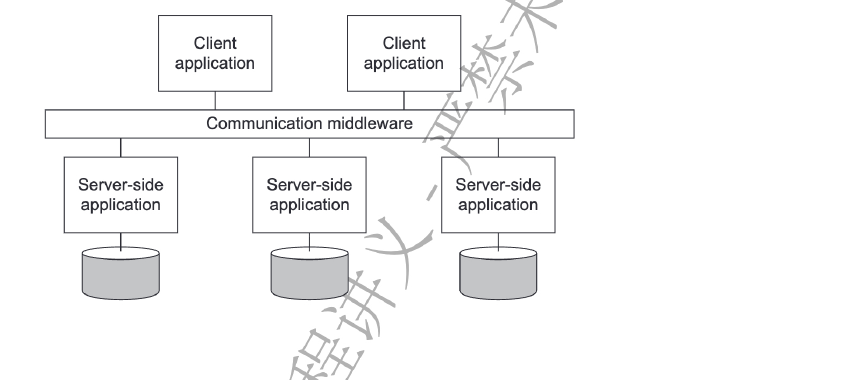
\includegraphics[width=0.68\textwidth]{figures/ch1/communication-middleware.png}
\caption{通过通信中间件连接客户端应用和服务端应用}
\end{figure}

\subsection{透明性}

\subsubsection*{透明性}

\begin{itemize}
  \item \textbf{透明性：}\blue{对用户和应用程序隐藏系统组件的物理分布性。}
  \item \textbf{理想目标：}\blue{使分布式系统使用体验接近单机系统。}
\end{itemize}

\begin{figure}[H]
\centering
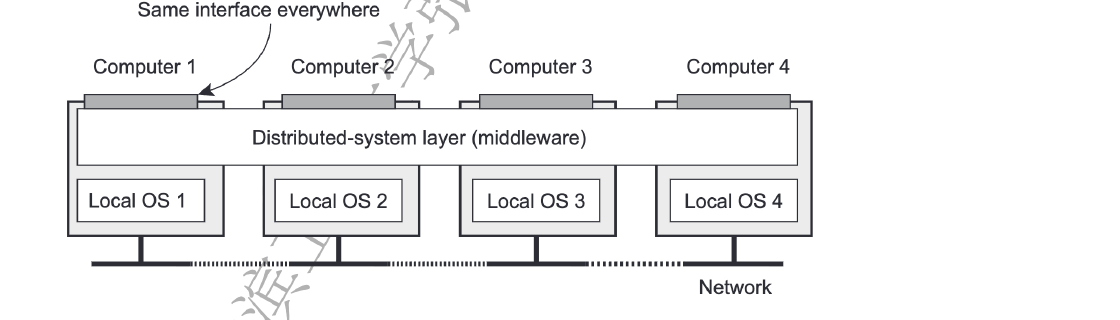
\includegraphics[width=0.78\textwidth]{figures/ch1/distributed-system-layer.png}
\caption{分布透明性的内涵}
\end{figure}

\paragraph{实现透明性：中间件}
位于 OS 与应用间的软件层，提供分布式系统共性服务。被称为：分布式系统的操作系统。典型技术：
\begin{itemize}
  \item 远程过程调用（RPC）：封装网络通信，支持同步/异步调用。
  \item 面向消息的中间件（MOM）：消息发送到逻辑联系点（发布），并转发给订阅的应用程序。
\end{itemize}

\paragraph{实现透明性：虚拟化}
\begin{figure}[H]
\centering
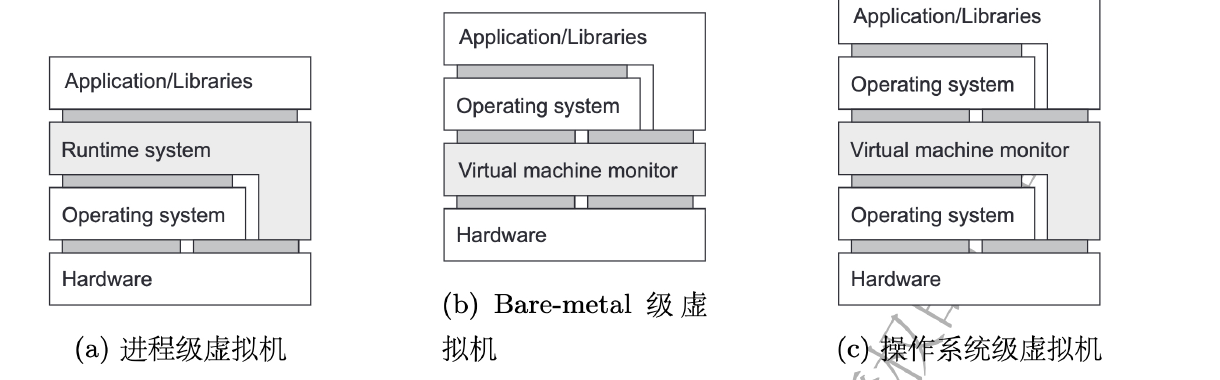
\includegraphics[width=0.88\textwidth]{figures/ch1/virtualization-types.png}
\caption{进程级、Bare-metal 级与操作系统级虚拟机}
\end{figure}

\begin{itemize}
  \item 核心优势：
  \begin{itemize}
    \item 支持计算迁移与负载均衡
    \item 故障/安全隔离
  \end{itemize}
\end{itemize}

\paragraph{透明性 $\ne$ “完全隐身”}
\begin{itemize}
  \item 追求“绝对透明”可能适得其反：系统会为“假装是单机”付出过高代价（如性能下降、复杂度飙升）。
  \item “绝对透明”可能只是个梦：
  \begin{itemize}
    \item 故障 vs. 慢
    \begin{itemize}
      \item 服务器没回消息，是崩溃了？还是卡在垃圾回收？
      \item 发微信：对方不回，是手机没电了，还是在装没看见？
    \end{itemize}
    \item 操作到底执行没？不确定！
    \begin{itemize}
      \item 服务器收到请求后刚写日志，就断电了……操作成功了吗？
      \item 网络超时重传？可能重复执行！
    \end{itemize}
  \end{itemize}
\end{itemize}

\paragraph{有时，“暴露分布性”更好}
敢说实话，反而更可靠、更高效：
\begin{itemize}
  \item 明确故障提示：“连接超时（30 秒无响应）”比“卡住不动”更友好。用户可选择：重试 / 换节点 / 稍后再试。
\end{itemize}

\paragraph{核心思想}
\blue{透明性是目标，但不是教条，平衡易用性、性能与可靠性才是关键。}

\subsection{开放性}

\subsubsection*{开放性}

\blue{系统通过标准化接口与协议支持互操作与集成。}要求：
\begin{itemize}
  \item 符合开放标准（如 HTTP, gRPC, OpenAPI）
  \item 支持跨平台应用互操作
  \item 保障应用可移植性
  \item 便于功能扩展
\end{itemize}

\subsection{可信任性}

\subsubsection*{可信任性}

\blue{可信任性（Dependability）的四大内涵：}

\begin{table}[H]
\centering
\caption{可信任性的核心要求}
\begin{tabularx}{\textwidth}{>{\raggedright\arraybackslash}p{0.34\textwidth}X}
\toprule
\textbf{要求} & \textbf{描述} \\
\midrule
\blue{可用性}（Availability） & 准备好供使用 \\
\blue{可靠性}（Reliability） & 服务交付的连续性 \\
\blue{安全性}（Safety） & 极低的灾难发生概率 \\
\blue{可维护性}（Maintainability） & 故障系统修复的难易程度 \\
\bottomrule
\end{tabularx}
\end{table}

\paragraph{故障、错误与失效}

\begin{table}[H]
\centering
\caption{故障、错误与失效}
\begin{tabularx}{\textwidth}{>{\raggedright\arraybackslash}p{0.22\textwidth}X>{\raggedright\arraybackslash}p{0.2\textwidth}}
\toprule
\textbf{术语} & \textbf{描述} & \textbf{示例} \\
\midrule
\blue{故障}（Fault） & 系统中可能导致失效的异常\textbf{源头} & 软件 Bug \\
\blue{错误}（Error） & 故障后导致的内部不正确\textbf{状态} & 内存越界 \\
\blue{失效}（Failure） & 系统对外表现出的不符合规格的\textbf{表现} & 停止服务 \\
\bottomrule
\end{tabularx}
\end{table}

\paragraph{术语：处理缺陷}
\begin{table}[H]
\centering
\caption{处理缺陷的术语}
\begin{tabularx}{\textwidth}{>{\raggedright\arraybackslash}p{0.24\textwidth}X>{\raggedright\arraybackslash}p{0.18\textwidth}}
\toprule
\textbf{术语} & \textbf{描述} & \textbf{示例} \\
\midrule
\blue{预防}（Prevention） & 防止故障的发生 & 代码审查 \\
\blue{容错}（Fault tolerance） & 故障（Fault）发生系统依然可正常运行的能力 & 冗余、副本 \\
\blue{消除}（Elimination） & 减少故障的存在、数量或严重性 & 补丁更新 \\
\blue{预测}（Prediction） & 估计故障的未来发生率和后果 & 压力测试 \\
\bottomrule
\end{tabularx}
\end{table}

\subsection{安全性}

\subsubsection*{安全性}

\blue{安全是可靠性的必要前提。}核心需求：
\begin{itemize}
  \item \blue{保密性}（Confidentiality）：信息仅向授权方披露
  \item \blue{完整性}（Integrity）：确保对系统资产的更改只能以授权方式进行
  \item \blue{可用性}（Availability）：防止服务拒绝（与可靠性交叉）
\end{itemize}

\paragraph{安全性机制}
授权（Authorization），认证（Authentication），信任（Trust）
\begin{itemize}
  \item \blue{认证：}验证声称的身份的正确性
  \item \blue{授权：}确定已认证实体的访问权限
  \item \blue{信任：}一个实体可以确信另一个实体将根据特定期望执行特定操作
\end{itemize}

\subsection{可扩展性}

\subsubsection*{可扩展性}

\begin{itemize}
  \item \blue{规模可扩展性}（Size scalability）：支持用户/节点/资源数量增长
  \item \blue{地理可扩展性}（Geographic scalability）：跨地域部署与低延迟访问
  \item \blue{管理可扩展性}（Administrative scalability）：支持多自治域策略协同
  \item 挑战：地理与管理可扩展性仍是主要瓶颈。
\end{itemize}

\paragraph{地理可扩展性的难点}
\begin{itemize}
  \item 高延迟破坏同步交互模型（如 RPC 超时）
  \item WAN 链路丢包率高不可靠，影响流媒体等实时应用
  \item 广播不可行，需专用命名/目录服务（如 DNS, LDAP）
  \item 时钟同步精度不完美，影响事件排序
\end{itemize}

\paragraph{管理可扩展性的难点}
\begin{itemize}
  \item 本质：\blue{关于使用、管理和安全的策略冲突}
  \item 模范示例：部分 P2P 系统（如 BitTorrent, 早期 Skype）依赖用户自发协作或严格的分布式协议，实现管理可扩展。
\end{itemize}

\paragraph{扩展技术 I：应对通信延迟}
\begin{itemize}
  \item 异步通信与非阻塞 I/O
  \item 回调（Callback）或 Future/Promise 模式
  \item 限制：需应用逻辑支持异步模型
\end{itemize}

\paragraph{扩展技术 II：云边端协同应对服务器和通信负载}
\begin{itemize}
  \item 将计算卸载至客户端或边缘节点
  \item 减轻服务器负载，提升响应速度
\end{itemize}

\begin{figure}[H]
\centering
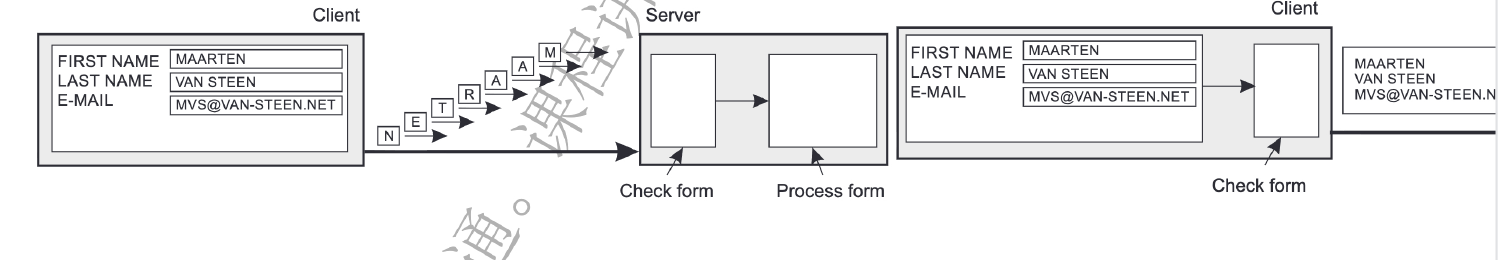
\includegraphics[width=\textwidth]{figures/ch1/client-server-form.png}
\caption{客户端与服务器协同处理表单}
\end{figure}

\paragraph{扩展技术 III：复制与缓存}
\begin{itemize}
  \item 复制：强一致性副本（如数据库主从）
  \item 缓存：弱一致性副本（如 CDN、浏览器缓存）
  \item 典型应用：
  \begin{itemize}
    \item 镜像站点
    \item Web 代理缓存
    \item 文件缓存（在服务器和客户端）
  \end{itemize}
\end{itemize}

\paragraph{复制的问题}
\begin{itemize}
  \item 有多个副本（缓存或复制）会导致不一致：修改一个副本会使该副本与其他副本不同。
  \item 始终保持副本与主副本完全同步需要全局同步每个修改，如何实现并提高效率？
\end{itemize}

\section*{结束语}
汇报完毕，欢迎同学们批评指教！本次课大致对应课程教材第一章。


\chapter{命名服务}
\section*{转写说明}
\addcontentsline{toc}{section}{转写说明}
原 PDF 为图片型长页，无可提取文本层。本文按视觉内容逐页转写为可编译的 \LaTeX{} 文档；原讲义中的长图、跨页图和示意图已从页面图像中裁切为独立插图，并按 A4 页面宽度与高度自动约束排版。

\section{实体与命名基础}

\subsection{实体与名字}

\paragraph{实体}
\begin{itemize}
  \item 主机、打印机、磁盘、文件；
  \item 进程、用户、邮箱、新闻组；
  \item 网络、页面等。
\end{itemize}

名字用来标识实体和指向实体的位置。

要对实体进行操作，我们需要在访问点访问它。接入点是通过地址命名的实体。

实体可拥有多个访问点，访问点随时间可能变化，如移动主机。

\subsection{名字 vs. 地址 vs. 标识符}

在计算机中称呼实体有很多方法，包括名字、地址和标识符：
\begin{itemize}
  \item \textbf{名字（Name）}：用于标注实体的字符串，如 \texttt{/etc/passwd}。
  \item \textbf{标识符（Identifier）}：系统内部唯一引用，本质是满足如下性质的名字：
  \begin{itemize}
    \item 一个标识符最多引用一个实体；
    \item 每个实体最多由一个标识符引用；
    \item 永久绑定：一个标识符始终引用同一个实体。
  \end{itemize}
  \item \textbf{地址（Address）}：访问点（部分特殊实体）的标识，含网络层（IP）与传输层（端口号），例如 \texttt{192.168.1.10:80}。
\end{itemize}

\subsection{属性与查找}

实体具有一组属性，形如 \(\langle\text{类型}, \text{值}\rangle\) 对。

例如打印机可以有：
\[
\langle\text{型号}, \text{LaserJet Pro}\rangle,\quad
\langle\text{类型}, \text{彩色}\rangle
\]

属性可用于查找实体。

\section{命名机制}

\subsection{命名机制分类}

\begin{itemize}
  \item 扁平命名（Flat Naming）；
  \item 结构化命名（Structural Naming）。
\end{itemize}

\subsection{扁平命名（Flat Naming）}

扁平命名：标识符只是随机的比特串，我们将其称为非结构化名称或扁平名称。

如何解析扁平名称，即仅凭标识符定位实体：
\begin{itemize}
  \item \textbf{广播}：广播 ID，让实体返回它的当前地址。只能在本地网络进行，且实体必须保持监听并及时回应。例：ARP 协议（IP 地址 \(\to\) MAC）。
  \item \textbf{向前指针}：地址变化后维护一个指向下个地址的指针。通过简单地跟踪指针链，可以实现对客户端完全透明的解引用。问题是地理可扩展性差，需要单独的链缩减机制；长链不具备容错性；会增加网络延迟。
  \item \textbf{“基站”方法（home-based approaches）}：实体的基站在命名服务机构存档。基站中记录实体的最新地址。要查询首先联系命名服务机构，再查阅基站。基站的地址永久不变，且负责实体的整个生命周期，灵活性差。
\end{itemize}

\begin{figure}[H]
  \centering
  \figimg{figures/ch2/fig01-home-based.png}
  \caption{基于基站的方法：先把包发送到主机的家乡位置，返回当前位置地址，再把包隧道转发到当前位置，后续包直接发往当前位置。}
\end{figure}

\subsection{分布式哈希表（DHT）}

分布式哈希表（DHT）是将标识符解析为关联实体的地址的最典型应用之一。
\begin{itemize}
  \item 在 P2P 网络（如 BitTorrent）或分布式缓存（如 Dynamo、Cassandra）中运用。
  \item 资源和节点都映射为一个固定长度的扁平位串。
  \item 多个节点组织成一个逻辑环：
  \begin{itemize}
    \item 每个节点都被分配一个随机的 ID；
    \item 每个实体都对应唯一的 Key；
    \item Key 为 \(k\) 的实体属于 \(ID \ge k\) 的最小节点的管辖范围，称为 \(succ(k)\)。
  \end{itemize}
  \item \red{注意这里的实体和节点是两个概念。}
  \item 目的：\blue{沿环搜索，以通过 \(k\) 找到 \(succ(k)\)}。
  \item 但是如果沿着环逐个线性搜索，就太低效了。
\end{itemize}

\paragraph{DHT Chord 的简单演示}
\begin{itemize}
  \item 每个节点 \(p\) 维护一个最多 \(m\) 个条目的表格 \(FT_p[]\)：\(FT_p[i]=succ(p+2^{i-1})\)。
  \item 第 \(i\) 个条目 \(FT_p\) 指向距离 \(p\) 至少 \(2^{i-1}\) 个索引位置的第一个节点。
\end{itemize}

\begin{figure}[H]
  \centering
  \figimg{figures/ch2/fig02-chord-panel.png}
  \caption{Chord 环与 finger table 示例：图中展示实际节点、每个节点的 finger table，以及从节点 28 解析 \(k=12\)、从节点 1 解析 \(k=26\) 的路径。}
\end{figure}

\paragraph{DHT Chord 查询规则}
\begin{itemize}
  \item 要查 \(k\)，节点 \(q\) 将请求转发给节点 \(q\)，其在 \(FT_p\) 中的索引 \(j\) 满足 \(q=FT_p[j]\le k < FT_p[j+1]\)。
  \item 如果 \(p < k < FT_p[1]\)，则请求也会转发给 \(FT_p[1]\)。
\end{itemize}

\subsection{扁平命名 -- 层次化位置服务}

构建一个大规模搜索树，其底层网络被划分为多个层级域。每个域由一个单独的目录节点表示。最低级别的域称为叶域，通常对应于计算机网络中的局域网。

\begin{figure}[H]
  \centering
  \figimg{figures/ch2/fig04-location-domain-tree.png}
  \caption{层次化位置服务中的域、目录节点与位置记录。顶级域 \(T\) 包含子域 \(S\)，叶域位于层级底部。}
\end{figure}

层次化位置服务中：
\begin{itemize}
  \item 实体 \(E\) 的地址存储在叶节点或中间节点中。
  \item 该节点的父节点（更高层）会记录一个“指针”，指向包含该实体的子区域。
  \item 根节点知道所有实体的信息。
\end{itemize}

\paragraph{查询过程}
\begin{itemize}
  \item 从本地的叶子结点开始查询。
  \item 如果在当前层级没找到，就向更高层查询。
  \item 一旦找到记录了该实体指针的节点，查询就沿着指针向下“落”，最终定位到实体。
\end{itemize}

\begin{figure}[H]
  \centering
  \figimg{figures/ch2/fig05-location-lookup.png}
  \caption{层次化位置服务的查找：本地节点无实体记录则上行到父节点；节点知道实体所在方向时，将请求转发给子节点。}
\end{figure}

像 Google Spanner 或 CockroachDB 这种跨全球部署的数据库，在处理数据副本的定位时，会利用层级化的拓扑（Region \(\to\) Zone \(\to\) Node）来优化延迟。

\subsection{结构化命名（Structural Naming）}

\subsubsection{命名机制分类}

\begin{itemize}
  \item 扁平命名（Flat Naming）；
  \item \blue{结构化命名（Structural Naming）}。
\end{itemize}

\subsubsection{命名图}

命名图（Naming Graph）通常为 DAG（有向无环图）。叶节点表示一个名字实体，目录节点是一个引用其他节点的实体。

\paragraph{路径与名称}
\begin{itemize}
  \item \blue{绝对路径}：从根节点开始，如 \texttt{/remote/vn}；
  \item \blue{相对路径}：从当前节点开始；
  \item \blue{全局名称}：唯一标识实体；
  \item 局部名称：依赖上下文。
\end{itemize}

\begin{figure}[H]
  \centering
  \figimg{figures/ch2/fig06-naming-graph.png}
  \caption{命名图示例：节点 \(n1\) 存储 \texttt{elke}、\texttt{max}、\texttt{steen} 等条目；\texttt{/home/steen/keys} 指向节点 \(n6\)。}
\end{figure}

\subsubsection{命名空间（Name Space）}

基本操作：
\begin{itemize}
  \item \blue{命名解析}：根据名字查找其属性（主要为地址）；
  \item 增加名字项与绑定（实体加入）；
  \item 删除名字项与绑定（实体离开）；
  \item 修改名字项与绑定（实体迁移）。
\end{itemize}

\subsubsection{命名空间挂载（Mounting）}

命名空间挂载可将外部命名空间子树透明地挂接到本地某目录节点。

\begin{itemize}
  \item \blue{挂接点（Mount Point）}：存放外部访问信息的目录节点。
  \item 挂载需指定三项信息：
  \begin{enumerate}
    \item 访问协议名称，如 NFS、FTP；
    \item 服务器名称，如 \texttt{flits.cs.vu.nl}；
    \item 外部空间中被挂载的路径，如 \texttt{/home/steen}。
  \end{enumerate}
  \item 例：机器 B 的 \texttt{/home/steen} 挂接到机器 A 的 \texttt{/remote/vn}。
\end{itemize}

\begin{figure}[H]
  \centering
  \figimg{figures/ch2/fig07-mount-foreign-space.png}
  \caption{命名空间挂载：机器 A 中的挂接点保存 \texttt{nfs://flits.cs.vu.nl/home/steen}，引用机器 B 中的外部命名空间。}
\end{figure}

\paragraph{结构化命名：NFS 中的命名（1）}
\begin{itemize}
  \item 服务器可以导出其文件系统的一部分，然后不同的客户端可以通过挂载导入。
  \item 示例：网络文件系统。
\end{itemize}

\begin{figure}[H]
  \centering
  \figimg{figures/ch2/fig08-mount-nested-dirs.png}
  \caption{NFS 挂载嵌套目录：多个客户端把服务器导出的目录挂载到各自本地命名空间中。}
\end{figure}

\paragraph{结构化命名：挂载嵌套目录}
\begin{itemize}
  \item 示例：网络文件系统。
\end{itemize}

\begin{figure}[H]
  \centering
  \figimg{figures/ch2/fig09-transitive-mounting.png}
  \caption{传递式挂载示意：客户端从服务器 A 导入目录，服务器 A 又从服务器 B 导入子目录。}
\end{figure}

\section{命名服务器结构}

\begin{itemize}
  \item \blue{命名空间是由命名服务器实现与管理的}。
  \item 命名服务器由\textbf{数据库 + 解析软件}构成。
\end{itemize}

\paragraph{组件角色}
\begin{itemize}
  \item 客户：发起请求。
  \item 命名代理（Name Resolver）：客户端与服务器间的接口；负责缓存、协调。
  \item 命名服务器：管理绑定上下文、执行解析、与其他服务器通信。
  \item 命名解析上下文：含名字-地址绑定 + 额外信息（OS、架构等）。
\end{itemize}

\subsection{管理策略}

\begin{itemize}
  \item 集中式管理：单服务器管理全部上下文。优点：易实现、易管理；缺点：性能瓶颈、单点故障。
  \item 分布式管理：命名空间划分为多个域（zones），由多个服务器分担。优点：可扩展、容错性好；缺点：实现复杂。
  \item 多副本分布式管理：每个域有多个副本，如 NS1 与 NS4 同时存 Zone1。优点：负载均衡 + 高可用性。
\end{itemize}

\subsection{命名服务器功能}

命名服务器需支持以下操作：
\begin{itemize}
  \item \textbf{管理操作}：增 / 删 / 改目录项；权限控制。
  \item \blue{命名解析}：接收请求并返回地址。
  \item \textbf{缓存}：存储查询结果，加速后续访问。
  \item \textbf{多副本管理}：更新同步、一致性维护。
  \item \textbf{通信}：与命名代理、其他命名服务器交互。
  \item \textbf{数据库}：存储命名解析上下文或子域。
\end{itemize}

\section{命名解析方式}

\subsection{方式 I：迭代解析}

\blue{迭代解析（Iterative Resolution）}：
\begin{itemize}
  \item 服务器若不知答案，则返回“下一个应查询的服务器地址”；
  \item 客户 / 代理继续向该服务器查询；
  \item 通信开销大，但服务器负载轻。
\end{itemize}

\begin{figure}[H]
  \centering
  \figimg{figures/ch2/fig10-iterative-resolution.png}
  \caption{迭代解析示意：客户端解析器依次查询 root、nl、vu、cs 等命名服务器，并接收下一步查询信息。}
\end{figure}

\subsection{方式 II：递归解析}

\blue{递归解析（Recursive Resolution）}：
\begin{itemize}
  \item 服务器若不知答案，自行代客户继续查询；
  \item 最终将结果返回给客户；
  \item 服务器负载高，但客户通信轮次少；\textbf{缓存效果更佳}。
\end{itemize}

\begin{figure}[H]
  \centering
  \figimg{figures/ch2/fig11-recursive-resolution.png}
  \caption{递归解析示意：客户端只向初始服务器发起请求，后续查询由服务器之间代为完成。}
\end{figure}

\section{DNS 实例分析}

\subsection{DNS 命名空间}

\begin{itemize}
  \item 结构：倒置树形（根在顶部，无名）。
  \item 结点标号 \(\le 63\) 字符；全路径 \(\le 255\) 字符。
  \item 域名书写规范（右至左）：
  \begin{itemize}
    \item \texttt{flits.cs.vu.nl.}：末尾圆点表示根；
    \item \texttt{vu.nl} 是 \texttt{cs.vu.nl} 的父域。
  \end{itemize}
  \item 区域（Zone）：命名空间中由单一权威服务器管理的子树（不重叠划分）。
  \item 结点内容 = 一组资源记录（Resource Records, RR）。
\end{itemize}

\subsection{DNS 资源记录（RR）结构}

每条 RR 包含字段：
\begin{itemize}
  \item \textbf{Owner}：域名，如 \texttt{cs.vu.nl}；
  \item \textbf{Type}：16 位类型码；
  \item \textbf{Class}：16 位类别，通常为 IN = Internet；
  \item \textbf{TTL}：生存时间（秒）；
  \item \textbf{RDATA}：资源数据，格式依 Type 而定。
\end{itemize}

\paragraph{常见 Type 编码}
\begin{table}[H]
\centering
\begin{tabular}{@{}lll@{}}
\toprule
Name & Code & Meaning \\
\midrule
A & 1 & IPv4 address \\
NS & 2 & Name server \\
CNAME & 5 & Canonical name (alias) \\
SOA & 6 & Start of Authority \\
PTR & 12 & Pointer (for reverse lookup) \\
MX & 15 & Mail exchange \\
TXT & 16 & Text \\
\bottomrule
\end{tabular}
\caption{DNS 常见资源记录类型。}
\end{table}

\subsection{域名服务器类型}

三类 DNS 服务器：
\begin{itemize}
  \item \textbf{根域名服务器（Root Name Server）}：返回顶级域（TLD）服务器地址。
  \item \textbf{本地域名服务器（Local Name Server）}：客户默认查询点。
  \item \textbf{授权域名服务器（Authoritative Name Server）}：对某 zone 有权威回答权，当本地域名服务器不知道时会查询它。
\end{itemize}

\subsection{顶级域（TLD）分类}

\paragraph{机构域（Generic TLDs）}
\begin{itemize}
  \item \texttt{.com} -- commercial；
  \item \texttt{.edu} -- educational；
  \item \texttt{.gov} -- government；
  \item \texttt{.org} -- non-profit；
  \item \texttt{.net} -- network provider；
  \item \texttt{.mil} -- military；
  \item \texttt{.biz}、\texttt{.info}、\texttt{.aero} 等。
\end{itemize}

\paragraph{地理域（Country Code TLDs）}
\begin{itemize}
  \item \texttt{.cn} -- China；
  \item \texttt{.uk} -- United Kingdom；
  \item \texttt{.jp} -- Japan；
  \item \texttt{.de} -- Germany；
  \item \texttt{.fr} -- France；
  \item \texttt{.au} -- Australia。
\end{itemize}

\subsection{DNS 查询与解析}

\begin{itemize}
  \item \blue{名称解析}：将域名 \(\leftrightarrow\) IP 地址。
  \item \blue{查询方式}：
  \begin{itemize}
    \item \blue{迭代查询}：服务器返回“下一个服务器地址”，由请求方继续查询；
    \item \blue{递归查询}：服务器代为完成全程查询，返回最终结果。
  \end{itemize}
  \item \blue{正向解析}：域名 \(\to\) IP（最常见）。
  \item \blue{逆向解析}：IP \(\to\) 域名，通过 PTR 记录，如 \texttt{in-addr.arpa} zone。
\end{itemize}

\subsection{结构化命名：现代 DNS}

\begin{itemize}
  \item DNS 实现的传统组织 vs DNS 的现代组织。
\end{itemize}

\begin{figure}[H]
  \centering
  \figimg[width=.86\linewidth]{figures/ch2/fig12-modern-dns.png}
  \caption{现代 DNS 架构：多个客户端可以经本地 resolver 访问互联网中的多个 name server。}
\end{figure}

\begin{figure}[H]
  \centering
  \figimg[width=.86\linewidth]{figures/ch2/fig13-traditional-dns.png}
  \caption{传统 DNS 架构：客户端经 resolver 与互联网上的命名服务器交互。}
\end{figure}

\section{总结}

\begin{itemize}
  \item 命名服务是分布式系统的基础设施。
  \item 核心问题：命名 \(\to\) 属性，尤其是地址。
  \item 命名空间为分层 DAG，支持挂载与扩展。
  \item DNS 是典型实现：分层、分区、多副本、缓存优化（现代 DNS）。
  \item 解析策略权衡：迭代 vs. 递归；集中 vs. 分布式。
\end{itemize}

汇报完毕，欢迎同学们批评指教！本次课大致对应课程教材第六章。


\chapter{通信}
\section{目录}

\begin{enumerate}
\item 通信的维度
\item 远程过程调用 (RPC)
\item 基于消息的通信
\item 组播通信 (Multicast Communication)
\end{enumerate}

\section{通信的维度}

\begin{itemize}
\item \textbf{编码/解码 (marshaling)}
\item \textbf{命名与发现 (naming)}
\item \textbf{安全 (authentication/encryption)}
\item \textbf{扩展性机制 (replication, caching)}
\item \textbf{应用层协议}：业务特定专属逻辑
\end{itemize}

\bigskip
\hrule
\bigskip

\textbf{通信的两个核心维度}：生命周期与同步性

\begin{itemize}
\item \textbf{生命周期}
  \begin{itemize}
  \item \textbf{持久 (Persistent)}
  \item \textbf{瞬时 (Transient)}
  \end{itemize}
\item \textbf{同步性}
  \begin{itemize}
  \item \textbf{同步 (Synchronous)}
  \item \textbf{异步 (Asynchronous)}
  \end{itemize}
\end{itemize}

\begin{table}[htbp]
\centering
\begin{tabular}{@{}lll@{}}
\toprule
模型 & 发送方与接收方行为 & 典型技术 \\
\midrule
同步 + 瞬时 & 阻塞等待响应 & HTTP, gRPC, TCP RPC \\
同步 + 持久 & 阻塞等待入库确认 & e.g., 2PC, ZooKeeper \\
异步 + 瞬时 & 立即返回（无确认） & e.g., UDP, ZeroMQ \\
异步 + 持久 & 立即返回（后台重试） & RabbitMQ, Kafka \\
\bottomrule
\end{tabular}
\end{table}

\textbf{核心洞察}：
\begin{itemize}
\item \textbf{生命周期}决定：消息是否在中间件持久存储。
\item \textbf{同步性}决定：发送方是否需要等待接收方处理结果。
\end{itemize}

\subsubsection{生命周期 —— 消息能“活”多久？}

\begin{itemize}
\item \textbf{瞬时通信 (Transient)}
  \begin{itemize}
  \item 消息不存储：若下一跳不可达则丢弃。
  \item 示例：UDP datagram, Go RPC (Channel)。
  \end{itemize}
\item \textbf{持久通信 (Persistent)}
  \begin{itemize}
  \item 消息持久化存储，直至成功投递。
  \item 示例：RabbitMQ, Kafka, Email (MTA 队列)。
  \end{itemize}
\end{itemize}

\subsubsection{同步性 —— 发送后是否等待？}

\begin{itemize}
\item \textbf{异步通信 (Asynchronous)}
  \begin{itemize}
  \item 发送后立即返回，不阻塞。
  \item 需额外机制获取结果（回调/轮询/事件）。
  \item 示例：RocketMQ 事务消息, Kafka Producer。
  \end{itemize}
\item \textbf{同步通信 (Synchronous)}
  \begin{itemize}
  \item 发送后阻塞等待，直到收到应答。
  \item 编程模型简单（似本地函数）。
  \item 示例：Go RPC Call(), HTTP 请求-响应。
  \end{itemize}
\end{itemize}

\textbf{被动接收}：指不轮询，依赖中间件推送或事件驱动（如 Listener/Callback）。

\section{远程过程调用 (RPC)}

\subsubsection{RPC 基本原理}

\begin{itemize}
\item \textbf{动机}：让远程通信像调用一个本地函数一样简单，隐藏通信细节。
\item \textbf{核心思想}：通过过程调用机制隐藏网络通信细节，实现隔离性、原子性。
\end{itemize}

\begin{figure}[htbp]
\centering
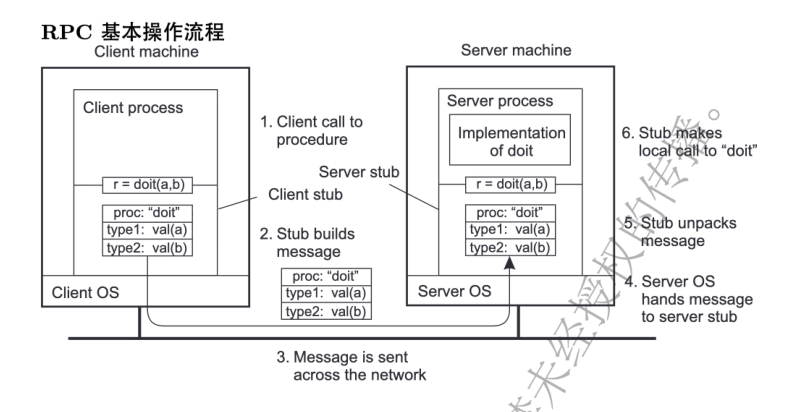
\includegraphics[width=0.8\textwidth]{figures/ch3/ch3_rpc_flow.png}
\end{figure}

（图：RPC 调用流程示意，客户端调用本地过程，由 Stub 封装网络通信，服务端 Stub 调用实际过程并返回结果）

\subsubsection{RPC 的故障语义}

\begin{itemize}
\item \textbf{核心难点}：客户端无法区分“请求未达”与“已处理但应答丢失”。
\item \textbf{常见语义}：
  \begin{itemize}
  \item \textbf{Best-effort}：超时重试，可能重复执行。
  \item \textbf{At-most-once}：绝不重试，保证操作不重复执行。
  \item \textbf{Exactly-once}：[疑似: 可能漏执行]。
  \end{itemize}
\end{itemize}

\section{基于消息的通信}

\subsubsection{Sockets}

\begin{itemize}
\item \textbf{BSD Socket API}：
  \begin{itemize}
  \item 关键操作：\texttt{socket()}, \texttt{bind()}, \texttt{listen()}, \texttt{accept()}, \texttt{connect()}, \texttt{send()}, \texttt{recv()}, \texttt{close()}。
  \item 特点：底层、灵活，但易出错；Client/Server 模式代码结构高度重复。
  \end{itemize}
\end{itemize}

\begin{figure}[htbp]
\centering
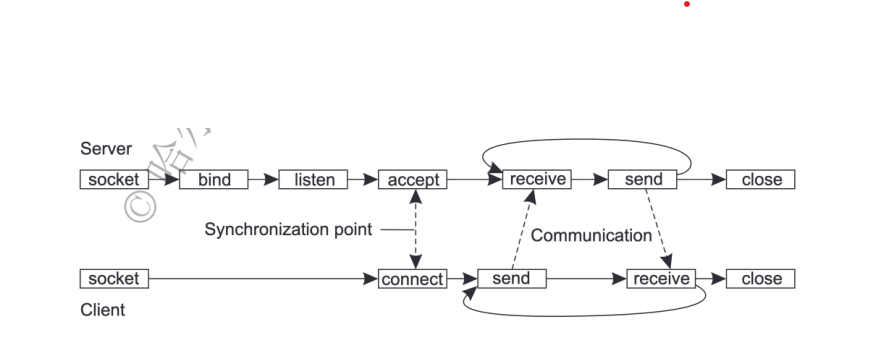
\includegraphics[width=0.8\textwidth]{figures/ch3/ch3_socket_flow.png}
\end{figure}

（图：Socket 通信流程。Server 端依次调用 socket, bind, listen, accept，然后阻塞在 receive；Client 端调用 socket, connect, send，最后 close。）

\textbf{改进}：Golang 等语言对 Socket API 进行了封装，但接收方仍需处理消息边界等问题。

\subsubsection{MOM (Message-Oriented Middleware)}

\begin{itemize}
\item \textbf{基本操作}：
  \begin{itemize}
  \item \textbf{PUT}：将消息追加至指定队列。
  \item \textbf{GET}：阻塞直至队列非空，并取出首消息。
  \item \textbf{POLL}：非阻塞检查并取首消息。
  \item \textbf{NOTIFY}：注册回调，消息到达时触发。
  \end{itemize}
\item \textbf{队列管理器 (Queue Manager)} 管理本地队列。应用仅能访问本地队列，跨节点的通信完全由 MOM 中间件自动完成。
\end{itemize}

\subsubsection{消息代理 (Message Broker)}

\begin{itemize}
\item \textbf{动机}：解决应用间消息格式异构问题。
\item \textbf{核心功能}：
  \begin{itemize}
  \item \textbf{转换 (Transformation)}：在不同协议/数据格式间转换。
  \item \textbf{应用网关 (Application Gateway)}：作为统一入口，提供协议适配、认证鉴权、负载均衡等服务路由。
  \item \textbf{基于主题的路由 (Subject-Based Routing)}：生产者向主题发布消息，消费者按需订阅。
  \end{itemize}
\end{itemize}

\subsubsection{标准协议：AMQP}

\begin{itemize}
\item \textbf{Advanced Message Queuing Protocol}：
  \begin{itemize}
  \item \textbf{基本模型}：
    \begin{itemize}
    \item \textbf{Connection}：稳定连接（TCP 级）。
    \item \textbf{Channel}：单向通道（轻量，可多个）。
    \item \textbf{Session}：会话管理。
    \item \textbf{Link}：基于 Socket，两个单向 Channel 构成。
    \end{itemize}
  \item \textbf{实现示例}：RabbitMQ。
  \end{itemize}
\end{itemize}

\section{组播通信 (Multicast Communication)}

应用层组播 (ALM)：
\begin{itemize}
\item \textbf{思想}：在节点间构建覆盖网络 (overlay network) 实现组播。
\item \textbf{拓扑}：
  \begin{itemize}
  \item 树状 (tree，高效)
  \item 网状 (mesh，需路由)
  \end{itemize}
\item \textbf{指标}：
  \begin{itemize}
  \item \textbf{Link stress}：同一物理链路被 ALM 流的占用情况。
  \item \textbf{Stretch}：ALM 路径延迟 / 物理最短路经延迟。
  \end{itemize}
\end{itemize}

\subsubsection{泛洪 (Flooding) 与优化}

\begin{itemize}
\item \textbf{基本泛洪}：节点向所有邻居广播消息 (除来源外)，且需记录已见消息。
\item \textbf{优化：概率泛洪 (Probabilistic Flooding)}
  \begin{itemize}
  \item 节点以概率 $p_{flood}$ 转发消息。
  \item $p_{flood}$ 可根据度数 (degree) 等动态调整。
  \end{itemize}
\end{itemize}

\subsubsection{Gossip 协议}

\begin{itemize}
\item \textbf{假设}：无写-写冲突。
\item \textbf{特点}：
  \begin{itemize}
  \item 更新操作仅在单个服务端上执行；
  \item 副本仅将更新后的状态传播给少数相邻节点；
  \item 传播是惰性的 (lazy)，即非即时进行；
  \item 最终，每次更新应到达所有副本（最终一致性）。
  \end{itemize}
\item \textbf{副本}：共享同一份数据（或状态）的多个节点实例。
\end{itemize}

\textbf{两类模型}：
\begin{itemize}
\item \textbf{Anti-entropy}：节点随机两两配对，交换状态差值。
\item \textbf{Rumor spreading}：更新节点主动“传染”若干邻居。
\end{itemize}

\subsubsection{Anti-entropy 模型}

\begin{itemize}
\item 节点 $P$ 随机选取系统中另一节点 $Q$，然后执行如下三类操作：
  \begin{itemize}
  \item \textbf{拉取 (Pull)}：$P$ 仅从 $Q$ 拉取其缺失的更新。
  \item \textbf{推送 (Push)}：$P$ 仅将自身新的更新推送给 $Q$。
  \item \textbf{双向 (Push-Pull)}：$P$ 与 $Q$ 互相交换更新。
  \end{itemize}
\item \textbf{性能}：$O(\log N)$ 轮可使全部 $N$ 个节点获知更新。
\item \textbf{概率分析（单源）}：
  \begin{itemize}
  \item Pull: $p_{k+1} = p_k^2$
  \item Push: $p_{k+1} \approx p_k e^{-1}$
  \item Push-pull: $p_{k+1} \approx p_k^3$
  \item 推导见教科书。
  \end{itemize}
  （其中 $p_k$ 为第 $k$ 轮后仍未获知更新的节点比例）
\end{itemize}

\subsubsection{Rumor Spreading 模型}

\begin{itemize}
\item \textbf{机制}：更新者 $s$ 逐个联系其邻居，将更新推送给他们。
\item 设 $s$ 为未知更新节点比例，$1/p_{stop}$ 为停止概率参数。
\item 理论推导可得剩余节点数随时间变化。
\item \textbf{示例}（$N = 10^5$，每次新推送 1 个节点，$p_{stop}=0.2$）：
  \begin{itemize}
  \item 第 1 轮仍有未更新概率：0.203，剩余约 20320 节点。
  \item 第 3 轮仍有未更新概率：0.0198，剩余约 1980 节点。
  \item 第 5 轮仍有未更新概率：0.0025，剩余约 250 节点。
  \item 第 7 轮仍有未更新概率：0.00034，剩余约 34 节点。
  \end{itemize}
\item \textbf{局限}：无法保证 100\% 覆盖，需结合其他机制（如 anti-entropy）。
\end{itemize}

\subsubsection{删除操作的挑战}

\begin{itemize}
\item \textbf{问题}：单纯删除某个值后，Gossip 传播反而可能将其恢复。
\item \textbf{解决方案}：引入\textbf{死亡证书 (death certificate)}。
  \begin{itemize}
  \item 将删除本身视为一种特殊更新，传播至所有副本，且操作必须 [疑似: 覆盖旧数据/具有更高优先级]。
  \end{itemize}
\item \textbf{死亡证书清理策略}：
  \begin{itemize}
  \item \textbf{全局算法}：检测全网已知后统一回收（类似 GC）。
  \item \textbf{乐观策略}：赋予最大生命周期（需承担遗漏风险）。
  \end{itemize}
\end{itemize}

\section{总结}

\begin{itemize}
\item \textbf{通信是分布式系统的基石}，需根据场景选型。
\item \textbf{RPC}：适合请求-应答模式，隐藏网络细节（但需处理故障）。
\item \textbf{Messaging}：适合解耦、异步、可靠投递。
\item \textbf{Multicast / Gossip}：适合大规模状态同步。
\item \textbf{关键原则}：删除操作必须谨慎处理，通常需引入特殊机制。
\end{itemize}

本次课大致对应课程教材第 2 章 [疑似: 第2章]。


\chapter{时间与逻辑时钟}
\section{时钟同步}

分布式编辑-编译工作流示例。例如：2144, < 2143。调用编译器则 make 不会重新编译，因为缺乏时间同步导致文件时间戳不匹配。

物理时钟。有时我们只需要精确的时间，而不仅仅是顺序。基于协调世界时(UTC)的时间信号，可通过短波/长波无线授时台、BERTIE SRS (GNSS)、RISNTTDRLY/(NTP/PTP) HRS 等方式向用户提供授时服务。

铯133原子无干扰的基态超精细能级间。(国际计量大会1967)。为什么跃迁对应辐射的9192631770个周期。

时间同步困难：
\begin{itemize}
\item 硬件时钟本身的不精确性。
\item 网络延迟，如消息延迟会使服务器应答过时。
\end{itemize}

\subsubsection{时钟同步：偏移与漂移}
时钟偏移：两个时钟值之间的相对差异。
时钟漂移：本地时钟相对‘完美参考时钟’的时间偏差现象。
时钟漂移率：本地时钟相对‘完美参考时钟’在单位时间内产生的时间偏差量。

\paragraph{Cristian's Algorithm 概述}
\begin{enumerate}
\item 客户端发送请求数据包，用其本地时钟打上时间戳 $T_1$。
\item 服务器用其本地时钟记录收到请求的时间 $T_2$。
\item 服务器发送响应数据包，包含其本地时钟 $T_3$ 和 $T_h$。
\item 客户端用其本地时钟记录收到服务器响应的时间 $T_4$。
\end{enumerate}

\paragraph{Cristian's Algorithm: 偏移量计算}
客户端采样往返时间 $\delta$：$\delta = (T_4 - T_1) - (T_3 - T_2)$。但客户端知道 $\delta$，不知道请求延迟 $req$ 和响应延迟 $resp$。假设 $req = resp = \delta/2$，则偏移量 $\theta = T_3 + \delta/2 - T_4$。

\begin{figure}[htbp]
\centering
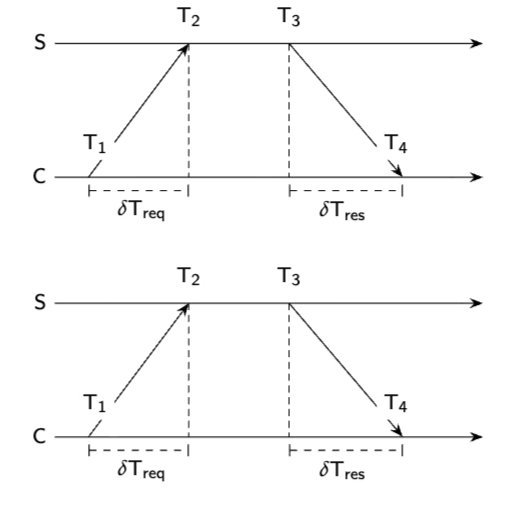
\includegraphics[width=0.8\textwidth]{figures/ch4/ch4_cristian_algorithm.png}
\caption{Cristian's Algorithm 往返时间计算示意}
\end{figure}

\begin{figure}[htbp]
\centering
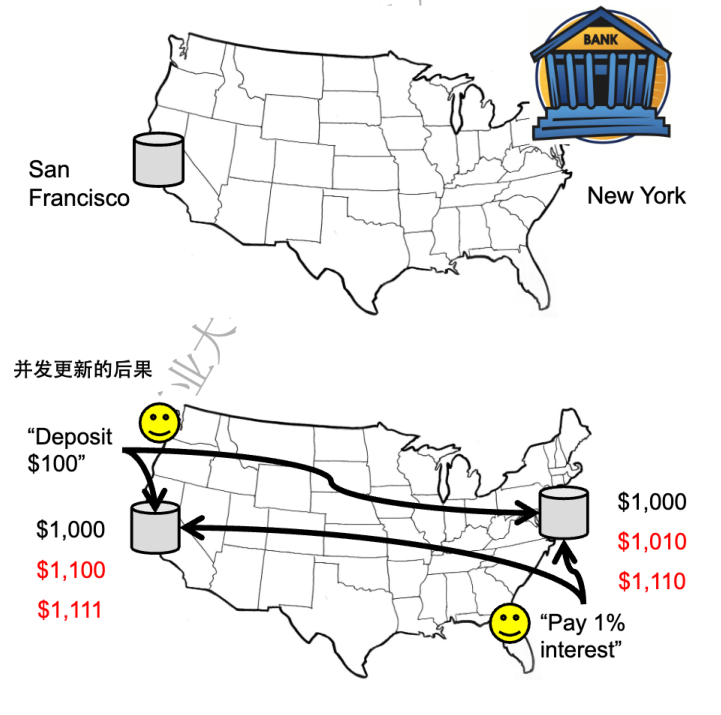
\includegraphics[width=0.8\textwidth]{figures/ch4/ch4_replica_inconsistency.png}
\caption{无协调下副本不一致示意}
\end{figure}

在无协调情形下，可能导致不一致的副本！更新应在每个副本上以相同的顺序执行。

\subsection{逻辑时钟}

\subsubsection{Lamport 逻辑时钟}

逻辑时钟。1978年Leslie Lamport的里程碑论文。洞察：只有事件顺序才是重要的，忽略精确的时间。捕获事件之间的“happens before”关系（$\to$ 关系）。通常重要的不是事件确切的时间，而是事件的发生顺序。

定义（$\to$）：
\begin{itemize}
\item 在同一进程中，如果事件 $a$ 发生在 $b$ 之前，则 $a \to b$。
\item 在不同进程中，如果 $a$ 是消息的发送，$b$ 是该消息的接收，则 $a \to b$。
\item 传递性：如果 $a \to b$ 且 $b \to c$，则 $a \to c$。
\end{itemize}

这在具有并发操作进程的系统中引入了事件偏序。
并发事件：并非所有事件都由 $\to$ 相关。$a$ 和 $b$ 不是由 $\to$ 相关，所以是并发的，记为 $a || b$。

\paragraph{Lamport 逻辑时钟}
问题：如何维护与“发生在之前”关系一致的系统行为的全局视图？
为每个事件 $e$ 附加一个时间戳 $LC(e)$，满足以下属性：
\begin{itemize}
\item P1: 如果 $a$ 和 $b$ 是同一进程中的两个事件，且 $a \to b$，则 $LC(a) < LC(b)$.
\item P2: 如果 $a$ 对应于消息 $m$ 的发送，$b$ 对应于该消息的接收，则 $LC(a) < LC(b)$.
\item P3: 对于所有事件 $a$ 和 $b$，如果 $a \to b$，则 $LC(a) < LC(b)$.
\end{itemize}

\paragraph{Lamport 逻辑时钟：实现规则}
每个进程 $P_i$ 维护一个本地计数器 $Clock_i$ 并调整：
\begin{enumerate}
\item 对于进程内发生的每个新事件，$Clock_i$ 增加1（属性P1）。
\item 每当进程 $P_i$ 发送消息 $m$ 时，消息时间戳 $LC(m) = Clock_i$（属性P2）。
\item 每当进程 $P_j$ 接收消息 $m$ 时，$P_j$ 将其本地计数器 $Clock_j$ 调整为 $\max(Clock_j, LC(m))$，然后在将 $m$ 传递给应用程序之前执行步骤1（属性P2）。
\end{enumerate}

两个事件仍可能同时发生。通过进程ID打破平局来避免这种情况。这里给大家板书演示一下。

\begin{figure}[htbp]
\centering
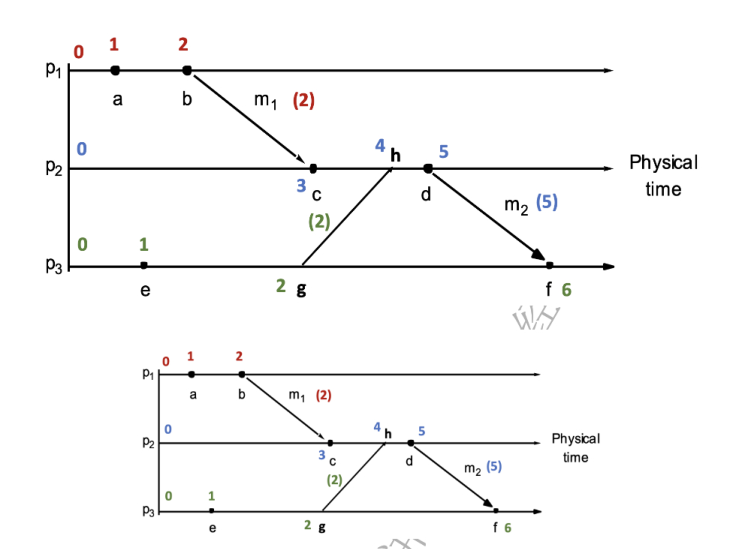
\includegraphics[width=0.8\textwidth]{figures/ch4/ch4_lamport_clock.png}
\caption{Lamport 逻辑时钟板书演示}
\end{figure}

一有两个副本。结果：在没有适当同步的情况下，副本\#1 为1111元，而副本\#2为1110元。

\subsubsection{全序多播推导（见板书）}

全序多播（ISIS）：
\begin{enumerate}
\item 发送阶段：发送者 $S$ 将一条消息 $M$ 多播给组内的所有接收者，这条消息被标记为“不可交付”（Undeliverable）。
\item 提议阶段（Bidding）：接收者 $P_i$ 收到消息 $M$ 后，查看每个本机最大序号记录（包括接收的和提议的），回复发送者一个“提议序号” $P_i = \max(\text{看到的最高序号}) + 1$。将 $M$ 放入一个优先级队列中，状态依然是“不可交付”，并暂时按提议序号排序。
\item 定标阶段（Selection）：发送者 $S$ 收集所有接收者返回的提议序号，从所有回复中选出最大值 $P_{max}$。这个 $P_{max}$ 就成为消息 $M$ 的最终序号。
\item 确认阶段（Commitment）：发送者 $S$ 再次多播一条确认消息，告诉所有人：“消息 $M$ 的最终序号是 $P_{max}$”。
\item 交付阶段（Delivery）：每个接收者收到确认消息后，将本地队列中消息 $M$ 的状态改为“可交付”，并按 $P_{max}$ 对队列重新排序。
\end{enumerate}

多站点复制的问题就这么容易的解决了吗？全序多播是否解决了多站点复制的问题？远非如此！我们的协议假设：无节点故障，无消息丢失，无消息损坏，All-to-all 通信不具扩展性，为消息延迟永远等待（性能差）。

\subsubsection{向量时钟}

Lamport时钟与因果关系。Lamport时钟时间戳可能无法捕获因果关系。即：不能保证如果 $LC(a) < LC(b)$，则 $a$ 因果上先于 $b$。给定 $LC(a)$ 和 $LC(z)$，我们想知道是否存在连接它们的事件链 $a \to \dots \to z$。

向量时钟：介绍。一个标量无法对多个进程中的事件进行排序，因而我们想将其扩展为一个向量。向量时钟 (Vector Clock) 是一个整数向量，分布式系统中每个进程都有一个。为事件 $e$ 标记 $VC(e) = [c_1, c_2, \dots, c_n]$。每个条目 $c_k$ 是进程 $k$ 中因果先于 $e$ 的事件计数。

\begin{figure}[htbp]
\centering
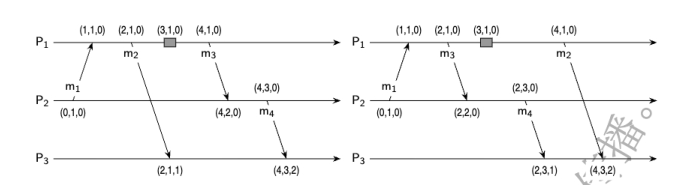
\includegraphics[width=0.8\textwidth]{figures/ch4/ch4_vector_clock.png}
\caption{向量时钟示例：多进程事件与向量时间戳}
\end{figure}

\paragraph{向量时钟：更新规则}
每个进程 $P_i$ 维护一个向量 $VC_i$：
\begin{itemize}
\item $VC_i[i]$ 是 $P_i$ 的本地逻辑时钟。
\item 如果 $VC_i[k] = k'$，则 $P_i$ 知道 $P_k$ 已经执行了 $k'$ 个事件。
\end{itemize}

初始时，所有向量都是 $[0,0,\dots,0]$。

两个更新规则：
\begin{enumerate}
\item 对于进程 $P_i$ 上的每个本地事件，执行前递增本地条目 $VC_i[i] := VC_i[i] + 1$。
\item 如果进程 $P_j$ 接收从 $P_i$ 发来的消息，并附带向量 $d = [d_1, d_2, \dots, d_n]$，则：
   \begin{itemize}
   \item 对每个 $k$，$VC_j[k] := \max(VC_j[k], d_k)$；然后 $P_j$ 递增自己的条目 $VC_j[j] := VC_j[j] + 1$。
   \end{itemize}
\end{enumerate}

交付给上层应用。

\paragraph{向量时钟：比较}
比较向量时间戳的规则：
\begin{itemize}
\item $VC(a) = VC(b)$ 当且仅当对所有 $k$, $VC(a)[k] = VC(b)[k]$，则 $a$ 和 $b$ 是同一事件。
\item $VC(a) < VC(b)$：对所有 $k$, $VC(a)[k] \le VC(b)[k]$，且存在 $k'$, $VC(a)[k'] < VC(b)[k']$，则 $a \to b$。
\item 并发性：如果存在 $i,j$，使得 $VC(a)[i] < VC(b)[i]$ 且 $VC(a)[j] > VC(b)[j]$，则 $a || b$。
\end{itemize}

\paragraph{比较Lamport时钟和向量时钟}
两个事件 $a$, $z$：
\begin{itemize}
\item Lamport时钟：$LC(a) < LC(z)$ 不能推导出 $a \to z$，即可能 $a \to z$ 或 $a || z$。
\item 向量时钟：$VC(a) < VC(z) \Rightarrow a \to z$。
\end{itemize}

拓展：向量时钟可以用来实现因果有序多播，即：确保仅当所有因果先于待交付消息的消息已被传递时才传递消息。例子：腾讯文档。

\paragraph{因果有序多播}
原则：如果消息A在逻辑上先于消息B产生，那么任何接收者都必须先处理A，再处理B。即保证所有存在happens-before关系的消息顺序。

实现方式：
\begin{itemize}
\item 发送端：当进程 $P_i$ 想要发送消息 $m$ 时：自增计数器 $VC_i[i] := VC_i[i] + 1$，不仅发送消息 $m$，还会把此时自己本地持有的整个向量 $[VC_i[1] \dots VC_i[N]]$ 附带在消息里。发送者在信封里塞了一张清单，告诉所有人：“这是我发的第 X 封信，在此之前，我已经收到了其他进程的这么多封信。”
\item 接收端：当进程 $P_j$ 收到来自 $P_i$ 的消息 $m$（附带有向量 $V$）时，它不会立即交付，而是先放在缓冲区，检查以下两个条件：
  \begin{enumerate}
  \item 消息序列连续性：$V[i] = VC_j[i] + 1$。这个消息必须是 $P_i$ 发出的“下一封”。
  \item 所有因果依赖都满足：对所有 $k \ne i$，$V[k] \le VC_j[k]$。即 $P_i$ 发出这封信之前，它所见过且来自其他所有进程的消息，$P_j$ 都已经接收并处理了。
  \end{enumerate}
\item 交付：当上述两个条件同时满足时：
  \begin{itemize}
  \item 提交：消息 $m$ 被正式交付给应用层（CO-deliver）。
  \item 更新状态：$VC_j[i] := V[i]$；对所有 $k$, $VC_j[k] := \max(VC_j[k], V[k])$。$P_j$ 记录下自己已经处理完 $P_i$ 的最新进展。
  \end{itemize}
\end{itemize}

全序多播是一种利用 Lamport 时钟实现分布式系统中事件全局排序的方法。全序多播协议需要仔细处理消息确认，以确保事件按正确顺序处理。尽管全序多播有用，但它假设了理想的网络和节点条件，且扩展性有限。

\begin{figure}[htbp]
\centering
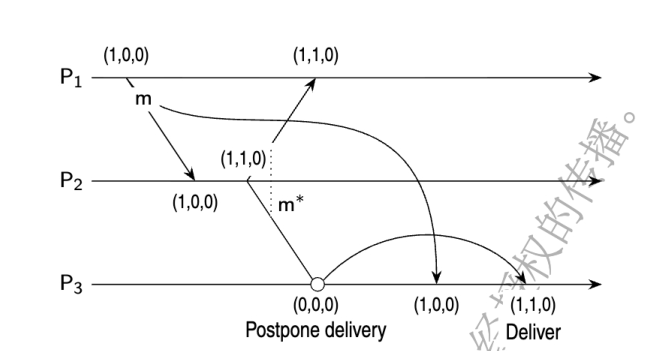
\includegraphics[width=0.8\textwidth]{figures/ch4/ch4_total_order_multicast.png}
\caption{全序多播协议流程}
\end{figure}

在分布式系统中可以对事件进行全序排序。根据构造，$a \to b$ 意味着 $LC(a) < LC(b)$ 一定成立。但命题的逆不成立：$LC(a) < LC(b)$ 不一定意味着 $a \to b$。注意不能使用Lamport时间戳来推断事件之间的因果关系。举例：Lamport时钟不能保证：如果 $LC(a) < LC(c)$，我们不能得出“$a$ 在因果上先于 $c$”。

逻辑时钟位于哪里？

示例应用：全序多播。
全序多播：所有消息都按相同的顺序传递给每个接收者。
复制数据库上的并发更新在各副本处以相同的Lamport时钟顺序执行。
例如：P1向账户添加100美元（初始值：1000美元）。
[图示：消息交付应用，复制数据库，物理时间轴...]


\chapter{互斥与选举算法}
本课程《分布式系统》指定QQ群（群号：1083024265）作为教学通知的官方发布平台。任课教师已于2026年4月3日课堂上正式宣布该安排，自宣布之日起，教师已履行教学告知义务。请全体选课学生及时加入该群并定期查阅通知；因个人未及时关注群内信息而影响作业提交或课程考核的，相关责任由学生本人承担。

\section{1 互斥：问题与基本方案}

\begin{itemize}
\item 问题：分布式系统中的多个进程需要独占访问某些资源。
\item 基本解决方案：
  \begin{itemize}
  \item 基于权限：想要进入临界区或访问资源的进程需要来自其他进程的权限。
  \item 基于令牌：令牌在进程之间传递。拥有令牌的进程可以在临界区中继续，或者在不感兴趣时传递它。
  \end{itemize}
\end{itemize}

\subsection{集中式算法}

\begin{itemize}
\item 使用协调器。
\item 协调器拥有共享资源的权限。权限被授予请求的进程。
\item 进程向协调器请求访问。
\item 如果另一个进程随后请求访问同一资源的权限，协调器不回复（直到前一个释放）。
\item 当进程释放资源时，它告诉协调器，协调器然后回复等待的下一个进程。
\end{itemize}

\subsection{Ricart \& Agrawala 算法}

与 Lamport 算法相同，除了不发送确认。

\begin{itemize}
\item 如果接收方没有访问该资源，并且也不想访问，它会向发送方发送一条 OK 消息。
\item 如果接收方已经可以访问该资源，它不会回复，而是将请求放入队列。
\item 如果接收方也想访问该资源，但尚未访问，它会将传入消息的时间戳与它发送给所有人的消息中的时间戳进行比较。时间戳较短的那个优先。
\item 如果传入消息的时间戳较短，接收方会发送一条 OK 消息；如果接收方自身的消息时间戳较短，接收方会将传入的请求放入队列，不回复。
\end{itemize}

\subsection{Ricart \& Agrawala 算法例子}

\begin{figure}[htbp]
\centering
\includegraphics[width=0.8\textwidth]{../work/figures/placeholder}
\caption{Ricart \& Agrawala 算法示例图}
\label{fig:ricart}
\end{figure}

\subsection{令牌环算法}

\begin{itemize}
\item 本质：将进程组织成逻辑环，让令牌在它们之间传递。拥有令牌的进程被允许进入临界区（如果它想的话）。构造为逻辑环的覆盖网络，带有循环令牌。
\end{itemize}

\subsection{ZooKeeper（互斥）}

\begin{itemize}
\item ZooKeeper 维护基于树的命名空间，类似于文件系统。
\item 锁定协议：客户端创建/删除节点以获取/释放锁。
\item 版本控制：用于防止竞争条件。
\end{itemize}

\section{2 选举算法}

\subsection{选举算法：原理}

\begin{itemize}
\item 许多系统要求某些进程充当协调器。问题是如何动态选择这个特殊进程。
\item 在许多系统中，协调器是手动选择的（例如集中式解决方案）。
\end{itemize}

\subsection{选举算法：基本假设}

\begin{itemize}
\item 所有进程都有唯一 ID。
\item 所有进程都知道系统中所有进程的 ID（但不知道它们是启动还是关机）。
\item 选举意味着识别启动的具有最高 ID 的进程。
\end{itemize}

\subsection{欺凌算法（Bully）}

\begin{itemize}
\item 原理：当进程注意到协调器不再响应请求时，它启动选举：Px 向所有具有更高标识符的进程发送选举消息。
\item 如果没有人响应，它赢得选举并成为协调器。
\item 如果上级之一回答，它接管，它的工作完成。
\end{itemize}

\begin{figure}[htbp]
\centering
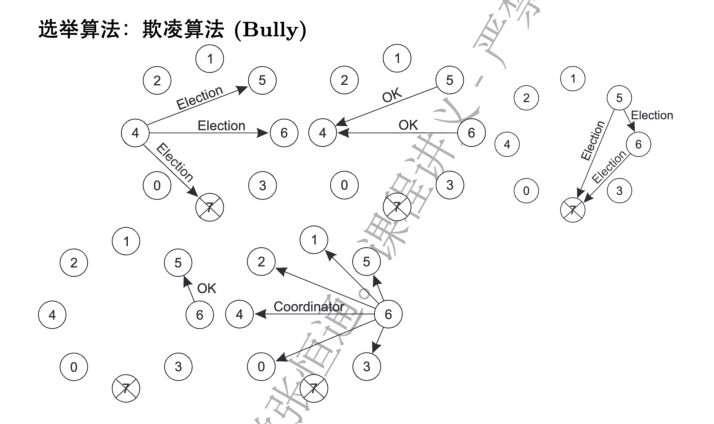
\includegraphics[width=0.8\textwidth]{figures/ch5/ch5_bully_algorithm.png}
\caption{欺凌算法示意图}
\label{fig:bully}
\end{figure}

\subsection{环算法}

\begin{itemize}
\item 基本思想：将所有进程按编号组织成一个逻辑环，通过环形传递消息完成选举。
\item 启动选举：任一进程发现协调者失效后，可主动发起选举，向环中下一位邻居发送 'Election' 消息，并附上自身编号。若下一位邻居失效，继续跳过。
\item 消息传递：每个收到 'Election' 消息的进程，将自身编号加入消息列表，继续向后转发；若消息回到发起者，说明已遍历全环，所有存活进程均已报到。
\item 确定协调者：发起者从收集到的编号中选出最大者，并广播 'Coordinator' 消息通知全体——新一轮协调者正式产生。
\end{itemize}

\begin{figure}[htbp]
\centering
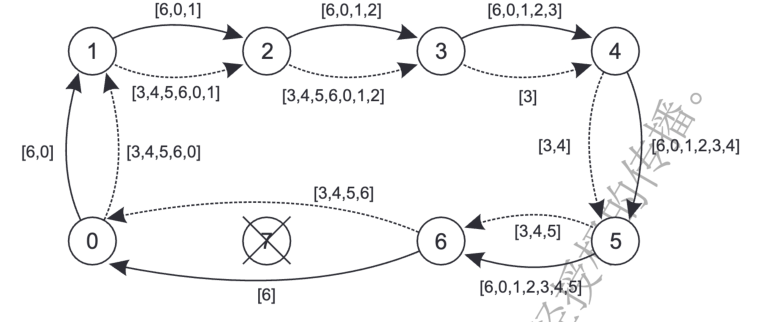
\includegraphics[width=0.8\textwidth]{figures/ch5/ch5_election_p6.png}
\caption{由 P6 发起的选举（实线）}
\label{fig:ring1}
\end{figure}

\begin{figure}[htbp]
\centering
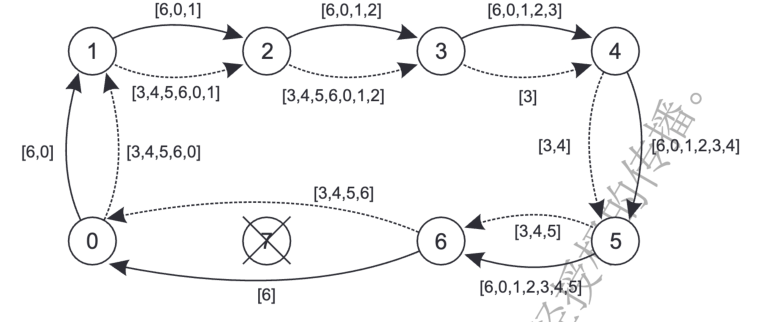
\includegraphics[width=0.8\textwidth]{figures/ch5/ch5_election_p3.png}
\caption{由 P3 发起的选举（虚线）}
\label{fig:ring2}
\end{figure}

图中实线表示由 P6 发起的选举，虚线表示 P3 发起的选举。该算法要求环结构场景。

\subsection{ZooKeeper 选举：PK 准则}

ZooKeeper 默认使用 Fast Leader Election 算法。当节点进入选举状态（LOOKING）时，遵循以下 PK 逻辑：

核心参数：
\begin{itemize}
\item ZXID (Transaction ID)：数据的新旧程度。越大的数据越新。
\item SID (Server ID)：服务器唯一编号。
\item Epoch：逻辑时钟，代表当前的选举轮次。
\end{itemize}

胜出判定（优先级由高到低）：
\begin{enumerate}
\item Epoch 优先：轮次大的直接胜出。
\item ZXID 优先：若轮次相同，数据越新的胜出。
\item SID 优先：若数据也一样新，SID 最大的胜出。
\item 注：当某个节点获得的票数超过集群总数的半数（$n/2 + 1$），即当选 Leader。
\end{enumerate}

\subsection{Fast Leader Election 算法逻辑}

每一个 ZooKeeper 节点在选举时本质上是一个状态机，其核心逻辑如下：

\begin{itemize}
\item 自增选举周期（logicalclock）：确保选举是在同一轮次进行的。
\item 初始化选票：初始状态下，每个节点都推举自己为 Leader。
\item 发送与接收：将选票广播给集群所有成员，并记录支持各投票的节点列表。
\item 收敛判定：每次更新投票后，节点统计集群中支持该投票的节点数。当某一个节点获得的票数过半，且没有更优的候选人出现时，选举终止。
\end{itemize}

状态：
\begin{itemize}
\item LOOKING：寻找 Leader 中。
\item LEADING：领导者状态。
\item FOLLOWING/OBSERVING：跟随者/观察者状态。
\end{itemize}

选举中的“见贤思齐”：为什么要改投？
在 LOOKING 状态下，每个节点都像是一个投票者。

第一阶段：自信投自己
每个节点启动时，都觉得自己是 Leader，发出一张选票：(SID, ZXID)

第二阶段：交换与动摇
收到别人的选票后，节点会进行思想斗争：
“它的数据（ZXID）比我新？”
“它的 ID 比我大？”
核心改投原则：只要对方展示出的“实力”（ZXID $>$ 我的，或 ZXID 相同但 SID 更大）比我强，我立刻撕毁旧选票，广播新选票，全心全意推举他。
结论：改投机制让选票迅速向“最强者”靠拢，实现快速收敛。

\subsection{选举流程：以5台服务器启动为例}

假设 5 台服务器 SID 分别为 1$\sim$5，按顺序启动：

\begin{table}[htbp]
\centering
\begin{tabular}{@{}ll@{}}
\toprule
启动顺序 & 选票变动与结果 \\
\midrule
Server 1 & 投自己 (1票) 票数未过半 (1/5)，等待 \\
Server 2 & Server 1 发现 2 的 SID 更大，改投 2，2号获得 2 票，未过半 \\
Server 3 & 1、2 发现 3 的 SID 最大，均改投 3，Server 3 晋升为 Leader \\
Server 4,5 & 发现已有 Leader，选举结束，直接以 Follower 身份加入 \\
\bottomrule
\end{tabular}
\caption{选举流程示例}
\label{tab:election}
\end{table}

\begin{itemize}
\item 崩溃恢复选举：当 Leader 宕机，其余节点进入 LOOKING，按上述 PK 流程重新选举。
\item 防脑裂：过半机制确保了全网只可能产生一个合法的 Leader 节点。
\end{itemize}

\subsection{经典选举与现代共识回顾}

基于 Bully 等算法：
\begin{itemize}
\item 假设：同步通信、无消息丢失、进程身份稳定；
\item 问题：一旦网络分区、消息延迟或节点反复宕机/重启，可能陷入：
  \begin{itemize}
  \item 活锁：多个进程/节点在不断尝试执行某个动作（如发起选举），但因互相干扰，导致谁都无法成功完成任务。
  \item 脑裂：系统中同时存在多个节点认为自己是协调者（Leader），并对外提供服务。
  \item 网络分区：网络故障导致集群分裂成多个子集，每个子集独立选出自己的 Leader，并继续处理请求。
  \end{itemize}
\end{itemize}

\subsection{经典选举与现代共识：现实挑战}

\begin{itemize}
\item 异步网络：消息延迟无上限（FLP 不可能性）；
\item 动态节点：节点随时加入/退出（如云环境）；
\item 状态一致性：不仅要选 Leader，更要保证状态一致！

且看：基于日志复制的共识协议（下章介绍）。
\end{itemize}

\bigskip

本次课汇报完毕。
欢迎大家批评指教。

对应课程教材第五章。


\chapter{一致性与复制}
\section{目录}

\begin{itemize}
\item 1 数据一致性模型
  \begin{itemize}
  \item 1.1 顺序一致性
  \item 1.2 线性一致性
  \item 1.3 因果一致性
  \item 1.4 最终一致性
  \end{itemize}
\item 2 客户端一致性模型
\item 3 副本管理 (对应 7.4 Replica management)
\end{itemize}

复制 (Replication) 为什么复制？
\begin{itemize}
\item 提高可靠性：如果一个副本失效，可以切换到另一个副本。
\item 提高性能与可扩展性：分散请求负载，或利用地理位置接近性实现快速响应。
\end{itemize}

现实问题：
\begin{itemize}
\item 拥有多个副本意味着当任何副本发生更改时，该更改必须在所有副本上执行。
\item 副本需要保持一致。
\end{itemize}

性能与可扩展性主要问题：
\begin{itemize}
\item 为了保持副本一致性，通常需要确保所有冲突操作在各处以相同顺序执行。
\item 冲突操作：来自事务领域的概念。
  \begin{itemize}
  \item 读-写冲突：读操作和写操作并发执行。
  \item 写-写冲突：两个并发写操作。
  \end{itemize}
\end{itemize}

挑战：保证不发生冲突操作的全局排序可能代价高昂，会降低可扩展性。
解决方案：弱化一致性要求，以避免全局同步。

\section{数据一致性模型}

数据一致性模型
一致性模型：
\begin{itemize}
\item 分布式数据存储与进程之间的契约。
\item 精确说明在并发情况下读写操作的结果。
\end{itemize}

\begin{verbatim}
Process   Process   Process
  |         |         |
Local copy  Local copy  Local copy
  \         |         /
   Distributed data store
\end{verbatim}

符号约定
读写操作符号：
\begin{itemize}
\item $W_i(x)a$：进程 $P_i$ 向数据项 $x$ 写入值 $a$。
\item $R_i(x)b$：进程 $P_i$ 从数据项 $x$ 读出值 $b$。
\end{itemize}
所有数据项初始值为 NIL。

示例：$P_i: W(x)a \;\rightarrow\; P_j: R(x)\text{NIL} \;\rightarrow\; R(x)a$

\subsection{顺序一致性}

顺序一致性 (Sequential Consistency) 定义：
\begin{itemize}
\item 所有结果需等同于所有进程按某种特定顺序执行，且
\item 该顺序执行结果要和每个进程自己代码里写的操作顺序一致。
\end{itemize}

例子：一个共享的在线文档，虽然每个人的更新到达时间可能不同，但系统最终会保证所有人看到的修改历史是同一个顺序 (比如：A 先改，然后 B 改，然后 C 改)，并且 A 的修改一定发生在 B 之前，B 在 C 之前。

顺序一致性示例。三个并发进程 (初始值: 0)：
\begin{itemize}
\item P1: x = x + 1; print(y, z);
\item P2: y = y + 1; print(x, z);
\item P3: z = z + 1; print(x, y);
\end{itemize}

执行序列：

\begin{verbatim}
Execution 1   Execution 2   Execution 3   Execution 4
P1: x=1;      P1: x=1;      P2: y=1;      P3: z=1;
P2: y=1;      P3: z=1;      P1: x=1;      P1: x=1;
P3: z=1;      P2: y=1;      P3: z=1;      P2: y=1;
print(x,y,z); print(x,y,z); print(x,y,z); print(x,y,z);
Prints: 001011  Prints: 101011  Prints: 010111  Prints: 111111
Signature:001011 | Signature:101011 | Signature:110101 | Signature:111111
 (a)             (b)              (c)              (d)
\end{verbatim}

小测验：看如下 P1 与 P2 并发的例子：这个运行结果满足顺序一致性吗？不满足，因为我们无法找到某个能产生这样效果的全局序。

\subsection{线性一致性}

线性一致性 (Linearizability) 定义：
\begin{itemize}
\item 每个操作都应该看起来在其开始和完成之间的某个时刻瞬间生效。
\end{itemize}

与顺序一致性的区别：
\begin{itemize}
\item 线性一致性要求操作具有实时性 (原子性)，即操作的效果看起来是瞬间发生的。
\item 顺序一致性只要求操作的最终顺序，不要求实时性。
\item 线性一致性 = 顺序一致性 + 实时性约束。要求每个操作在调用与返回之间的某个“瞬间”原子生效，且跨进程的操作顺序必须与真实时间先后严格一致。
\item 顺序一致性只要求：所有节点看到相同的全局操作总序；该顺序不违反单个进程内的程序执行顺序。不要求符合跨进程的真实时间先后。
\end{itemize}

示例对比：

\begin{table}[htbp]
\centering
\caption{线性一致性示例}
\begin{tabular}{ll}
\toprule
Result & Possible ordering of operations \\
\midrule
R1(x)b | R2(y)b & W1(x)a; W1(y)a; W2(y)b; W2(x)b \\
R1(y)b | R2(x)a & W1(x)a; W2(y)b; W1(y)a; W2(x)b \\
R1(x)b | R2(y)a & W1(x)a; W2(y)b; W2(x)b; W1(y)a \\
R1(y)b | R2(x)a & W2(y)b; W1(x)a; W1(y)a; W2(x)b \\
R1(x)b | R2(y)a & W2(y)b; W1(x)a; W2(x)b; W1(y)a \\
R1(x)a | R2(y)a & W2(y)b; W2(x)b; W1(x)a; W1(y)a \\
\bottomrule
\end{tabular}
\end{table}

\subsection{因果一致性}

因果一致性 (Causal Consistency)：
\begin{itemize}
\item 潜在因果相关的写操作必须被所有进程以相同顺序看到。
\item 并发的写操作可能被不同进程以不同顺序看到。
\end{itemize}

(a) 因果不一致的数据存储 (因为 P2 的 R(x)a 对 W(c)b 产生影响，所以 W(a)a -> W(c)b)
\begin{verbatim}
P1: W(x)a
P2: R(x)a  W(x)b
P3: R(x)a  R(x)b
P4:        R(x)a R(x)b
\end{verbatim}
(b) 因果一致的数据存储
\begin{verbatim}
P1: W(x)b
P2: R(x)b R(x)a W(x)b
P3: R(x)a R(x)b
P4: R(x)a R(x)b
\end{verbatim}

可串行化 / 事务可串行化 (serializability)：对一组事务中的所有操作进行排序，使得最终结果与这些事务的某种串行执行相匹配。

示例：
\begin{verbatim}
BEGIN_TRANSACTION
x=0
x=x+1
END_TRANSACTION

BEGIN_TRANSACTION
x=0
x=x+2
END_TRANSACTION

BEGIN_TRANSACTION
x=0
x=x+3
END_TRANSACTION

Transaction T1  Transaction T2  Transaction T3
A number of schedules
Time ->
S1 | x=0
S2 | x=0
S3 | x=0
S4 | x=0
x=x+1
x=0
x=0
x=0
x=x+2
x=x+1
x=x+1
x=x+2
x=0
x=0
x=x+3
x=0
考虑数据
x=0
x=0
x=x+2
x=x+3 | Legal
x=x+3 | Legal
x=x+3 | Illegal
x=x+1
x=x+2 | Illegal
\end{verbatim}

\subsection{最终一致性}

最终一致性 (Eventual Consistency) 定义：
在某一时刻停止更新后，所有更新都会传播，使得所有副本存储相同数据 (直到再次出现更新)。

直观例子：分布式系统存储集合和并发写操作。最终所有副本收敛一致。

一致性模型对比：

\begin{table}[htbp]
\centering
\caption{一致性模型对比}
\begin{tabular}{llll}
\toprule
一致性模型 & 核心特征 & 示例 & 强度 \\
\midrule
线性一致性 & 操作实时性约束，符合真实时间，严格原子生效，跨进程 & 银行转账: ATM取款后，全球查询余额立刻同步。 & 极强 (Real-time) \\
顺序一致性 & 所有节点看到相同的全局总序，且不违反进程内顺序。 & 网络游戏：所有玩家看到的击杀顺序必须一致，虽然可能有延迟。 & 中 (Logical-time) \\
因果一致性 & 仅保证有因果关系的写操作在所有节点顺序一致。 & 论坛发帖：先看到主贴 (因)，后看到回复 (果)。 & 中 (Causal-order) \\
最终一致性 & 不保证中间读取得结果，但系统最终会收敛到一致。 & DNS 修改：全球各处生效时间不一。 & 弱 (No guarantee) \\
\bottomrule
\end{tabular}
\end{table}

\section{客户端一致性模型}

核心思想：不追求全局一致，只保证单个客户端访问这个分布式数据库时，在任意位置读取得结果与之前在另一位置离开时的状态一致，即数据对该客户端而言是一致的。具体包括以下内容：
\begin{itemize}
\item 单调读：读不会“时光倒流” (应当越读越新)
\item 单调写：写不会“顺序颠倒” (应当先写先到)
\item 读你所写：自己写的，自己立刻能读到
\item 读后写：基于读的写，存在于读之后更新读版本 (因果)
\end{itemize}

客户端一致性实现基本思想：
\begin{itemize}
\item 每个写操作由其源服务器分配全局唯一标识符
\item 为每个客户端跟踪两个写操作集：读集和写集。
\end{itemize}

实现：
\begin{itemize}
\item 单调读：客户端传递读集，服务器拉取更新并更新读集。
\item 单调写：客户端传递写集，服务器拉取更新、排序并执行写操作，更新写集。
\item 读你所写：客户端传递写集，服务器拉取更新并执行读操作，更新读集。
\item 读后写：客户端传递读集，服务器拉取更新、排序并执行写操作，更新写集。
\end{itemize}

\section{副本管理 (对应 7.4 Replica management)}

\subsection{副本放置 (Replica Placement)}

目标：从 $N$ 个可能位置中找出最佳的 $K$ 个位置。
策略：
\begin{itemize}
\item 选择平均客户端距离最小的位置。(计算量大)
\item 选择第 $K$ 大自治系统，并在连接最好的主机上放置服务器。(计算量大)
\item 在反映延迟的 $d$ 维几何空间中定位节点，识别密度最高的 $K$ 个区域并在每个区域放置服务器。(计算量小)
\end{itemize}

\subsection{内容复制 (Content Replication)}

副本类型：
\begin{itemize}
\item 永久副本 (Permanent replicas)：始终拥有副本的进程/机器，可以被视为构成分布式数据存储的初始副本集。
\item 服务器发起副本 (Server-initiated replica)：是数据存储的副本，其存在是为了提升性能，并且是由数据存储的所有者主动创建的。托管副本设施，客户端使用它。
\item 客户端发起副本 (Client-initiated replica)：根据客户端请求动态的进程 (客户端缓存)。本质上，缓存是一种本地存储来临时存储刚刚请求的数据副本。
\end{itemize}

\subsection{内容分发 (Content Distribution)}

方式：
\begin{itemize}
\item 传播更新通知/失效 (常用于缓存)。
\item 在副本间传输数据 (分布式数据库)：被动复制。
\item 传播更新操作到其他副本：主动复制。
\end{itemize}

推送 (Push) 与拉取 (Pull)：
\begin{itemize}
\item 推送：服务器发起，无论目标是否请求。
\item 拉取：客户端发起，客户端请求更新。
\end{itemize}

租约 (Leases)：
\begin{itemize}
\item 租约是一种契约，服务器承诺在租约到期前将更新推送给客户端。
\item 自适应租约到期时间：基于年龄、续订频率、服务器状态。
\end{itemize}

\subsection{管理复制对象}

目标：
\begin{itemize}
\item 防止对同一对象的多次调用并发执行。
\item 确保复制状态的所有更改都相同。
\end{itemize}

解决方案：
\begin{itemize}
\item 使用本地锁定机制序列化对象内部数据访问。
\item 需要确定性线程调度以确保状态更改一致。
\end{itemize}

汇报完毕，欢迎同学们批评指教！本次课大致对应课程教材第七章。

% 原文可能存在不完整语句：“库对你而言是一致的。具有节 | [疑似: 未完]”，已忽略。


\chapter{分布式共识概念}
\section{两将军问题}

\begin{table}[htbp]
\centering
\begin{tabular}{@{}lll@{}}
\toprule
army 1 \textbackslash{} army 2 & does not attack & attacks \\
\midrule
does not attack & nothing happens & army 2 defeated \\
attacks & army 1 defeated & city captured \\
\bottomrule
\end{tabular}
\end{table}

两将军问题期望：当且仅当军队2发动攻击时，军队1发动攻击。

两将军问题是分布式计算领域中关于“共识一致性”的经典思想实验（1975），它主要探讨的是信道不可靠的问题。

将军们如何决策？
\begin{enumerate}
\item 将军1总是攻击，即使没有收到回应？派送大量信使以增加送达概率。如果全部被俘，2号将军不知道这次攻击，所以1号将军失败。
\item 1号将军只有在收到2号将军的积极回应时才会攻击。
\end{enumerate}

\begin{verbatim}
general 1   general 2
army 1   messengers   army 2
\end{verbatim}

现在1号将军安全。只有2号将军的回应通过并交付至1号，1号才会发动攻击。2号处境同1号。

两将军问题理论上无解（在异步网络中无法达成绝对一致）。

拓展至拜占庭将军问题，由 Lamport 在1982年提出，多将问题升级到了节点不可靠（存在叛徒）的情况。

拓展至拜占庭将军问题 [疑似: 图片内容: general 1 said retreat!]

\begin{figure}[htbp]
\centering
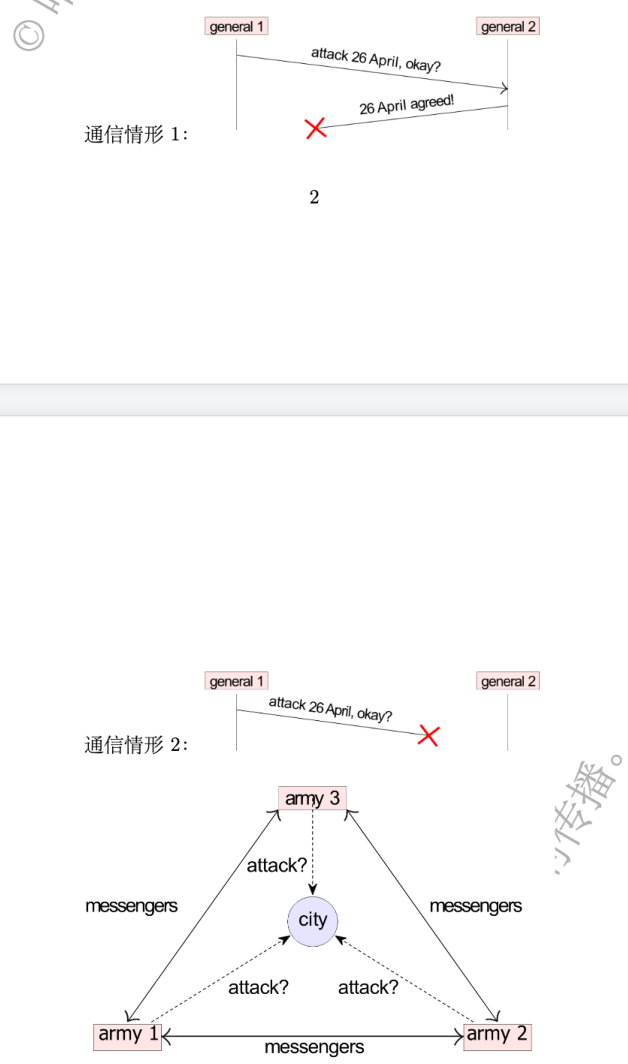
\includegraphics[width=0.8\textwidth]{figures/ch7/ch7_byzantine_generals.png}
\caption{拜占庭将军问题示意}
\end{figure}

\section{拜占庭将军问题的理论解}

假设：一共有 $n$ 位将军，其中包含诚实的将军与恶意的将军，多达 $f$ 名将军可能会有恶意行为；诚实的将军不知道谁是恶意的；恶意的将军们可能会串通密谋；尽管如此，诚实将军们务必达成一致计划。

结论：在消息能可靠传达的前提下，只要叛徒的数量满足 $n > 3f$（即诚实将军超过三分之二），共识就可以达成。（充要条件）

\section{分布式系统模型}

对系统模型进行假设，由以下三部分组成。

\subsection{网络模型}

假设两个节点之间进行双向点对点通信：
\begin{itemize}
\item 可靠链接：有发出就会被收到，但消息可能会被重新排序。
\item 公平-损失链接：是一种对“不完美网络信道”的抽象描述。会丢失、重复或重新排序，不断尝试终会收到。
\item 任意链接（活跃敌手）：恶意对手会干扰消息（窃听、修改、丢弃、欺骗、重放）。
\item 网络分区：在一个分布式系统中，由于网络故障，导致系统被分割成两个或多个互不通信的孤岛（子网）的现象。
\end{itemize}

\begin{quote}
Leslie Lamport, Robert Shostak, and Marshall Pease. 1982. The Byzantine Generals Problem. ACM Trans. Program. Lang. Syst. 4, 3 (July 1982), 382-401. \url{https://doi.org/10.1145/357172.357176}
\end{quote}

\subsection{节点模型}

节点有以下假设情况：
\begin{itemize}
\item 故障-停止：将永远停止执行。节点停止后，其他节点可以检测到其已停止。
\item 故障-恢复：丢失其在内存中的状态，可能会在稍后恢复执行。
\item 故障-省略 (Omission)：无法响应传入请求。
\item 故障-回复 (Response)：无法给出正确的响应。
\item 拜占庭节点，故障-随意 (fail-arbitrary)：故障节点可以[疑似: 做]任何事情，包括崩溃或恶意行为。
\end{itemize}

\subsection{同步模型}

同步假设如下：
\begin{itemize}
\item 同步：消息延迟不大于已知上限；节点以已知速度执行算法。
\item 部分同步：大部分时间是同步的，但在某些不可预知时刻，系统会进入异步。
\item 异步：[疑似: HERBIE. WARN BARRE.]
\end{itemize}

\section{3 CAP 定理}

\textbf{一致性 (C)}：系统中的所有节点都同意系统当前状态。

\textbf{可用性 (A)}：系统提供的服务必须一直处于可用状态，对于用户的每一个操作请求总是能够在有限时间内返回结果。

\textbf{分区容错性 (P)}：分布式系统在遇到任何网络分区故障（即节点间无法通信）时，仍能对外提供满足一致性或可用性的服务。

CAP 定理：在一个分布式系统中，一致性 (Consistency)、可用性 (Availability)、分区容错性 (Partition tolerance)，这三个要素最多只能同时实现两点，不可能三者兼顾。

\begin{figure}[htbp]
\centering
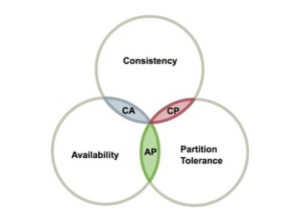
\includegraphics[width=0.8\textwidth]{figures/ch7/ch7_cap_theorem.png}
\caption{CAP 定理三者关系}
\end{figure}

\section{故障检测}

\begin{itemize}
\item 故障检测器：检测另一节点是否有故障的算法。
\item 发送消息，等待响应，若超时 [疑似: BAAR. MILAM.]。
\item 无法区分：崩溃节点、暂时无响应节点、丢失消息和延迟消息。
\end{itemize}

\begin{verbatim}
Periodic ping (Cr)  ack (Ca)
Periodic Cr) => Ca)
具体实现方法：每隔 T 给 p 发送 ping，等待 (T + Ac) 超时，若超时则疑似挂了。
同步情形：Δs = max network delay - min network delay
异步情形：Δs = k (observed delay); k > 1
\end{verbatim}

故障检测基于超时的完美故障检测器，仅存在于具有可靠链路、同步的崩溃-停止系统中。

最终完美故障检测器：
\begin{itemize}
\item 可能将节点临时标记为崩溃，即使它正确运行。
\item 可能将节点临时标记为正常的，即使它已经崩溃。
\item 但最终，将节点标记为已崩溃当且仅当它已崩溃。
\end{itemize}

实际情况：检测不会是即时的，可能会有虚假超时。

\section{故障模型}

\section{广播协议}

广播（多播）为组通信：
\begin{itemize}
\item 向所有节点发送消息，所有节点传递消息。（组成员集合可以是固定的（静态的）也可以是动态的。）
\item 如果一个节点出现故障，则其余组成员继续工作。
\end{itemize}

系统建模：
\begin{itemize}
\item 尽力交付：最大努力（可能会丢弃消息）。
\item 异步/部分同步时序模型：消息延迟没有上限。
\end{itemize}

\subsection{常见多播/广播顺序对比}

\begin{table}[htbp]
\centering
\begin{tabular}{@{}llll@{}}
\toprule
顺序类型 & 约束范围 & 典型场景 & 开销 \\
\midrule
FIFO 序广播 & 仅保证同一发送者的消息按发送顺序交付；不同发送者的消息无顺序保证 & 单源数据流、日志复制 & 最低 \\
因果序广播 & 保证所有存在因果依赖 (happens-before) 关系的消息按因果顺序交付；并发消息无强制顺序 & 协同编辑、聊天 & 中等（向量时钟） \\
全序广播 & 所有进程看到的全局交付顺序完全一致 & 分布式锁、多副本一致性 & 高（协调/共识协议） \\
FIFO-全序广播 & 同一发送者 FIFO 顺序基础上增加全局顺序约束；所有进程至全局交付顺序一致 & 分布式数据库、金融系统 & 高（共识算法与序列号校验） \\
\bottomrule
\end{tabular}
\end{table}

\subsection{广播协议演示}

\subsection{广播的现实问题}

\begin{itemize}
\item 网络异步性与延迟不确定性
\item 消息爆炸与带宽瓶颈
\item 消息乱序与重放 (Ordering \& Replay)
\item 节点成员变更的动态性
\item 拜占庭故障与安全性 (Byzantine Faults)
\end{itemize}

\section{FLP 不可能性}

分布式系统的一个根本问题是，如何在存在故障的情况下实现系统的整体可靠性。这通常需要协调各个进程以达成共识，即：就运行过程中所需的某些数据达成一致。

% image
% \includegraphics[width=0.8\textwidth]{../work/figures/placeholder}
% 请将 placeholder 替换为实际图片名称

在 FIFO 序基础上增加全局顺序约束：所有进程全局交付顺序一致，常见于分布式数据库、金融系统，开销高（共识算法与序列号校验）。


\chapter{Paxos}
\section*{目录}

\subsection{1 分布式共识回顾}

\textbf{什么是分布式共识：}每个进程都提出一个值。所有进程必须就其中一个提议值达成一致。

例子：
\begin{itemize}
\item 将军们必须就进攻时间达成一致
\item 分布式数据存储中跨多个服务器复制的对象，所有服务器必须就对象的当前版本达成一致
\item 在复制服务器上进行事务处理必须就对象更新的顺序达成一致
\end{itemize}

\subsection{FLP 定理}

\textbf{FLP 不可能性：}在异步-崩溃-停机系统模型中，不存在保证能终止的共识算法。

原文：
\begin{quote}
``The consensus problem involves an asynchronous system of processes, some of which may be unreliable. ... In this paper, it is shown that every protocol for this problem has the possibility of non-termination, even with only one possibly faulty process.''
\end{quote}
在一个完全异步的消息传递分布式系统中，其中即使只有一个发送崩溃故障，不可能存在达成共识的确定性算法。Fischer, Lynch 和 Paterson 在 1985 年著名的 FLP 不可能性结果中给予了证明。

\subsection{共识算法的设计目标}

一个完美的共识算法必须满足以下性质：
\begin{itemize}
\item \textbf{安全性 (Safety):} 任何时候都不会达成错误的共识（例如，两个不同的值被决议为‘共识’）。
  内涵包括：
  \begin{itemize}
  \item 一致性：所有诚实进程决定的值必须相同。 $\forall i, j \in \text{Correct}: d_i = d_j$。
  \item 确定性进程可能会：最终决定的值 $v$ 必须是由某个进程提出的初始值。 $v \in \{v_1, v_2, \dots, v_n\}$。
  \end{itemize}
\item \textbf{活性 (Liveness):} 不能陷入永久停滞。
  内涵为：
  \begin{itemize}
  \item 终止性 (Termination): 每一个诚实的进程最终都会在有限时间内完成决策。
  \end{itemize}
\end{itemize}

\subsection{FLP 定理的视角}

在完全异步系统中，没有任何确定性算法能同时严格满足上述两方面性质。
现有分布式共识算法如 Paxos 和 Raft 选择了在极端情况下牺牲 Liveness（活性）以绝对保证 Safety（安全性）。
为什么？如果强行要求活性，节点可能会在信息不足的情况下做出“猜测”，从而破坏安全性。

\section{2 Paxos}

\subsection{Paxos 共识算法}

异步系统中共识的 Paxos 算法。
\begin{itemize}
\item 最流行的共识算法。
\item Zookeeper, Google Chubby, 以及许多系统使用它。
\item 基本思想：一旦多数人同意一项提案，就达成共识。达成的共识最终为所有成员悉知。
\end{itemize}

猜猜是谁发明的？ Leslie Lamport! 原始论文: ``The Part-time Parliament''，使用了希腊 Paxos 岛上“兼职议会”的类比。该论文发表后难以理解。 1 年后发表了 ``Paxos made simple''。
参考：
\begin{itemize}
\item Leslie Lamport. The part-time parliament. ACM Transactions on Computer Systems (TOCS), Volume 16, Issue 2 Pages 133 -169
\item Leslie Lamport. (2001). Paxos Made Simple. ACM SIGACT News (Distributed Computing Column) 32, 4 (Whole Number 121, December 2001) pp. 51-58
\end{itemize}

\subsubsection{Paxos 共识算法: 角色划分}

角色: Paxos 将系统成员划分为三个角色: 提议者 (Proposer), 接受者 (Acceptor)，决策学习者 (Learner)

阶段: Paxos 算法决议过程包含三个阶段:
\begin{itemize}
\item 第一阶段: Prepare phase 准备阶段
\item 第二阶段: Accept phase 接受阶段
\item 第三阶段: Learn phase 学习阶段
\end{itemize}

提案: 包括提案编号 (Proposal ID) 和提议值 (Value); 提案指令，记为: $[n, v]$

\subsubsection{Paxos 共识算法: 提案编号}

允许接受者回应多个提案。
\begin{itemize}
\item 回应与接受：接受者 (Acceptor) 确实可以先后回复多个提案，但一旦某个提案被多数派 (Quorum) 接受，则达成共识，后续提案必须沿用该值。
\item 为不同进程配置不相交的可能提案编号集合。
\item 提案编号全序：高编号提案具有更高的优先级，可以令尚未达成的低编号提案失效。
\item 高编号会使接受者承诺不再批准任何低编号的提案（抢占）。
\item 如果提议者在准备阶段发现了已存在的值，它必须放弃自己的值，转而提议这个发现的高编号值。（确保 Safety）
\end{itemize}

\subsubsection{Paxos 共识算法: 三类角色}

三类角色（一个进程可以有多个角色）:
\begin{itemize}
\item 提议者 (Proposers): 向接受者提议值。
  \begin{itemize}
  \item 算法发起者，驱动协商进程
  \item 接受应用层请求，将请求封装为一个提案 (Proposal)
  \item 发送提案，将提案发送给所有接受者
  \item 根据响应，决定后续工作
  \end{itemize}
\item 接受者 (Acceptors): 接受提议的值 (在某些条件下)。
  \begin{itemize}
  \item 回应提议者的提案，根据规则进行投票表决。
  \item 处理: Prepare Request (准备请求) 和 Accept Request (接受请求)
  \item 选择: 多数 Acceptors 接受某 Accept Request，达成共识
  \end{itemize}
\item 学习者 (Learners): 学习已被多数接受者接受的值。
  \begin{itemize}
  \item 不参加提案发送与决策
  \item 采纳提议者/接受者最新达成一致的提案 (Value)
  \item 可根据实际需求，实现其它功能
  \end{itemize}
\end{itemize}

这里的多数意味着绝对多数（也包括崩溃的进程），假设崩溃的进程可以再次恢复。

\subsubsection{Paxos 算法: 尝试单阶段方案}

提议者将其提议的值组播到足够大的集合（大于多数派）的接受者。
\begin{itemize}
\item 接受者接受它收到的第一个提议值。如果多数接受者接受了相同的值 $v$，那么 $v$ 就是决定的值。
\item 这里可能会出什么问题？
  \begin{enumerate}
  \item 无法应对“提案冲突” (Race Condition)
  \item 无法处理“旧提案的滞后覆盖” (Stale Updates)，网络延迟是无法避免的
  \item 破坏安全性 (Safety Violation)
  \end{enumerate}
\end{itemize}

\subsubsection{Paxos: 算法 (Prepare 阶段)}

提议者: 选择一个提案编号 $M$，将 prepare request 发送给多数派接受者。$M$ 是全局唯一且单调递增的。

接受者: 收到 Prepare 请求后，根据规则响应:
\begin{itemize}
\item 如果 $M$ 大于此接受者已经回复的准备请求中的最大提案编号，则:
  \begin{itemize}
  \item 承诺在当前准备请求的响应中，不会回复并承诺任何编号较低的其他提案。
  \item 同时让提议者知道之前的共识状态: 反馈已接受的 Accept 请求中最大编号的提案指令；如果没有接受任何 Accept 请求，则反馈 Nil。
  \end{itemize}
\item 如果 $M$ 小于等于接受者已经回复的准备请求中最大提案编号，则拒绝本次 Prepare 请求，不回复提议者。
\end{itemize}

注意: 响应 Nil 和不响应并不相同。

\subsubsection{Paxos: 算法 (Accept 阶段)}

提议者: 如果提议者从多数接受者收到其准备请求 $M$ 的响应，则:
\begin{itemize}
\item 向每个这些接受者发送带有提议值的接受请求 (accept request)，请求包含提案编号和提案指令，记为 $[m, v]$。
\item 如果提议者没有听到多数接受者的响应怎么办？等待一段时间，然后发出带有更高编号的新请求。
\end{itemize}

接受者: 收到提案 $[m, v]$ 的接受请求后，根据以下约定对 Proposer 反馈:
\begin{itemize}
\item 如果接受者没有回复编号大于 $m$ 的 Prepare 请求，则接受提案 $[m, v]$，并返回已接受的最大编号。
\item 如果接受者已经回复编号为 $Y$ 的 Prepare 请求，且 $M < N$，则拒绝该 Accept 请求，回复 No。
\item 在下一轮协商中，提议者可以基于上述响应中的提案编号进行递增，而不用尝试逐个递增。
\item 如果多数接受者接受了该 Accept 请求，则记作提案 $[m, v]$ 已被选择或者达成共识。如果没有多数的接受者批准该 Accept 请求，则退回 Prepare 阶段重新协商。
\end{itemize}

\textbf{Paxos: 算法 (Accept 阶段) 中的值确定:}
\begin{itemize}
\item 如果在 Prepare 请求响应中，部分接受者反馈了提案指令，则 $v$ 为 Prepare 请求反馈中最大提案编号对应的提案指令，即使这不是提议者的初衷（保证“一旦选定，不可更改”）。
\item 否则，$v$ 可以由提议者任意指定。
\end{itemize}

\subsubsection{Paxos: 算法 (Learn 阶段)}

Learn 阶段不属于 Paxos 的协商阶段，将达成共识提案交给学习者，由其做相应操作。

学习者如何知晓已达成的共识提案?
\begin{enumerate}
\item 由 Proposer 同步: (最简方案) 只有提议者知道提案是否已达成共识和最终共识提案，如果已达成共识，Proposer 则立即将该提案发送给学习者。
\item 接受者转发 Accept 请求给学习者: 当接受者批准一个 Accept 请求时，将其转发给学习者，由其判断是否有多数接受者批准同一请求，以此决定如何操作（状态转移等）。
\item 接受者之间交换已批准的 Accept 请求: 当接受者批准一个 Accept 请求时，将其广播给其他接受者，则所有接受者都能判断提案是否已达成共识，并将共识提案发给学习者。明显又增加了一轮消息交互，但是，每个接受者都有已达成共识的标志，使得读请求不必再执行一轮协商。
\end{enumerate}

\subsection{Paxos 算法 FAQ}

如果我们有多个提议者怎么办?
\begin{itemize}
\item 两个提议者可能通过不断发送带有更高编号的新提案来抢占彼此的请求（活锁）。
\item 这里给大家演示一下活锁。
\item 安全性仍然得到保证!
\end{itemize}

如果多数接受者在值决定之前失败怎么办?
\begin{itemize}
\item 算法不终止。
\item 安全性仍然得到保证!
\end{itemize}

如果进程失败并再次恢复怎么办?
\begin{itemize}
\item 如果它是接受者，它必须记住它已接受的最高编号提案。接受者将接受的提案记录在磁盘上。
\item 只要此状态可以在故障和恢复后检索，算法就能正常工作，安全性仍然得到保证。
\end{itemize}

\subsection{日志共识}

\begin{itemize}
\item Paxos 算法（到目前为止讨论的）用于决定单个值。
\item 许多实际系统需要决定一系列值（日志）。
\item 复制日志 => 复制状态机。所有服务器以相同顺序执行相同命令。共识模块确保正确的日志复制。
\item 日志共识: Multi-Paxos: 对每个日志条目重复运行 Paxos。
  \begin{itemize}
  \item 很快变得非常复杂。
  \item 性能优化进一步增加了复杂性。
  \end{itemize}
\end{itemize}

\subsection{Paxos 的效率问题}

使用 Basic Paxos 效率较低:
\begin{itemize}
\item 多 Proposer 竞争
\item 多次 RPC (Prepare + Accept)
\end{itemize}
解决方案:
\begin{enumerate}
\item 选举 leader
\item 消除大多数 Prepare RPC
\end{enumerate}
优化方式:
\begin{itemize}
\item 对整个日志执行一次 Prepare（而不是每个条目）
\item 之后只运行 Accept
\end{itemize}

\subsection{Multi-Paxos 运行流程}

\subsubsection{阶段 A: Leader 选举 (Prepare)}
\begin{itemize}
\item 选择一个 Leader，并发送 Prepare(?, $m$)。
\item 一旦获得多数派承诺，该 Leader 拥有后续所有实例的写入权。
\end{itemize}

\subsubsection{阶段 B: 稳态运行 (Accept)}
\begin{itemize}
\item Leader 直接发送 Accept(I, $v$)
\item 响应耗时从 2-RTT 降低到 1-RTT。
\end{itemize}
注: 稳态下只需蓝色箭头的 Accept 阶段。

\begin{figure}[htbp]
\centering
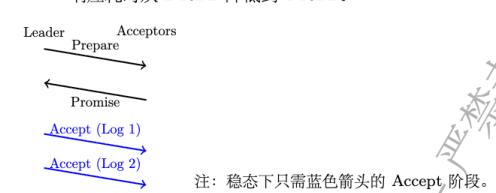
\includegraphics[width=0.8\textwidth]{figures/ch8/ch8_multipaxos_accept.png}
\caption{Multi-Paxos 稳态 Accept 阶段：Leader 向 Acceptors 复制日志}
\end{figure}

\subsection{总结}

\begin{itemize}
\item Basic Paxos: Prepare - Accept
\item Multi-Paxos: 包含 leader 选举、一次 Prepare、多次 Accept
\end{itemize}

\subsection{客户端协议、配置变更}

\subsection{对 Paxos 的批评}

\begin{quote}
``The dirty little secret of the NSDI community is that at most five people really truly understand every part of Paxos ;-).'' \hfill --- Anonymous NSDI Reviewer.
\end{quote}
\begin{quote}
``There are significant gaps between the description of the Paxos algorithm and the needs of a real-world system: ... the final system will be based on an unproven protocol.'' \hfill --- Chubby 作者
\end{quote}

\subsection{小结}

\begin{itemize}
\item 共识是分布式系统中的一个基本问题。
\item 可以在同步系统中解决共识。
  \begin{itemize}
  \item 基于时间同步轮次的算法。
  \item 需要至少 $(f+1)$ 轮来处理最多 $f$ 个故障。
  \end{itemize}
\item 不可能在异步系统中解决共识。
  \begin{itemize}
  \item 无法区分超时和非常非常慢的进程。
  \end{itemize}
\item Paxos 算法:
  \begin{itemize}
  \item 保证安全性但不保证活性。
  \item 希望在足够好的条件下终止。
  \end{itemize}
\end{itemize}

汇报完毕，欢迎同学们批评指教！
本次课涉及课程教材第?章，有大量补充内容。 % 需要指定章节


\chapter{PBFT}
\section{三阶段 作用}

Pre-prepare phase 和 Prepare phase (预准备和准备阶段) 用于确保所有节点在同一视图 (view) 下，并能够对请求进行全局排序，即使负责提议请求排序的主节点 (primary) 出现故障时也能保持一致性。

\begin{figure}[htbp]
\centering
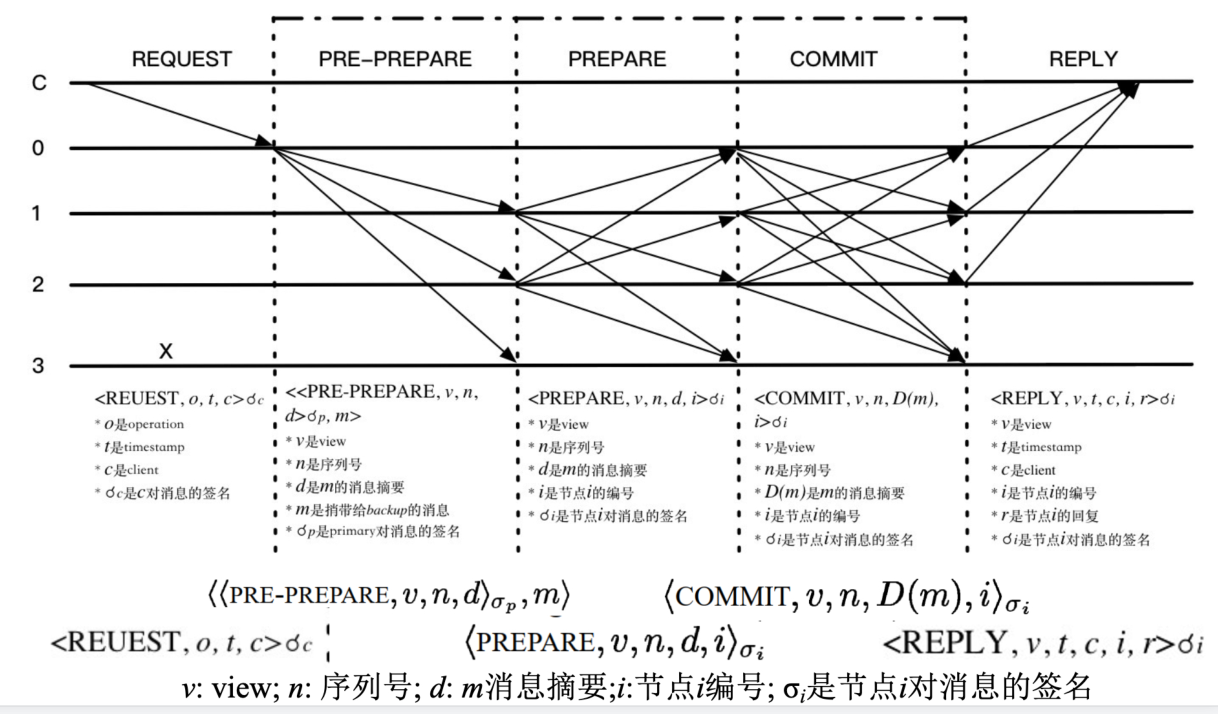
\includegraphics[width=0.8\textwidth]{figures/ch9/ch9_pbft_preprepare_prepare.png}
\caption{PBFT Pre-prepare 与 Prepare 阶段消息流程}
\end{figure}

\begin{table}[htbp]
  \centering
  \begin{tabular}{ccccc}
    \toprule
    & & 提交消息 [疑似: 给部分节点提交] & & \\
    \midrule
    节点 = & 1. 给所有节点广播正确的; 2. 给所有节点广播错误的; 3. 给部分节点广播错误的 & & \textasciitilde{} & 注意节点不切换 \\
    \bottomrule
  \end{tabular}
\end{table}

\subsection{View-change 阶段 (视图切换阶段)}

\begin{itemize}
  \item 有恶意节点 (最多 $f$ 个) 频繁发起视图切换
  \item 该进行视图切换时，恶意节点不切换
  \item 触发: 各节点只要收到 $f+1$ 个 View\_Change，自己便也发出 View\_Change。
  \item 达成: 新的主节点只要收到 $2f+1$ 个 View\_Change，即可发出 New\_View。
\end{itemize}

\subsection{PBFT 对比 Paxos}

\begin{itemize}
  \item PBFT 对比 Paxos，最大的不同在于解决的问题不一样
  \begin{itemize}
    \item 虽然都是共识算法，但一个解决的是拜占庭问题
    \item 另一个则解决的是非拜占庭问题
  \end{itemize}
  \item PBFT 中对应的主节点可能为恶意节点
  万一主节点作恶，从节点要有发现其是恶意节点的能力；
  并及时通过视图更换协议更换主节点
  \item BFT 需要从节点与从节点的消息交互
  只听主节点肯定是不行的，还要看看其他节点的意见；
  才有足额的节点认为是对的，就同意。
  \item 算法耗资源方面
  \begin{itemize}
    \item 明显 PBFT 要更复杂，投票数明显多
    \item [疑似: 内存占用、带宽开销更大]；
  \end{itemize}
  相比之下，[疑似: 其他共识算法(如 Paxos/ZAB) 在 PBFT 面前开销更小]。
\end{itemize}

\subsection{总结 PBFT 优点 vs. 缺点}

\subsubsection{优点:}

\begin{itemize}
  \item 首个实用的 BFT 共识容错算法，使得复杂度从指数级降低到多项式级 $O(n^2)$；
  \item 响应性 (Responsiveness): 在网络状况 OK，主节点不犯错，拜占庭节点数量不超过 $f$ 个时，在下一个视图一定是可以达成共识的。
\end{itemize}

\subsubsection{缺点:}

\begin{itemize}
  \item 通信复杂度 $O(n^2)$，可扩展性低；
  \item 视图转换的复杂度 $O(n^3)$，若考虑主节点和拜占庭节点，视图转换复杂度 $O(f n^3)$；
  \item 视图转换期间只能接收 view\_change、new\_view 消息，不能对外提供服务；
  \item Safety 和 Liveness 属性需要通过视图转换来保障。
\end{itemize}

\begin{figure}[htbp]
\centering
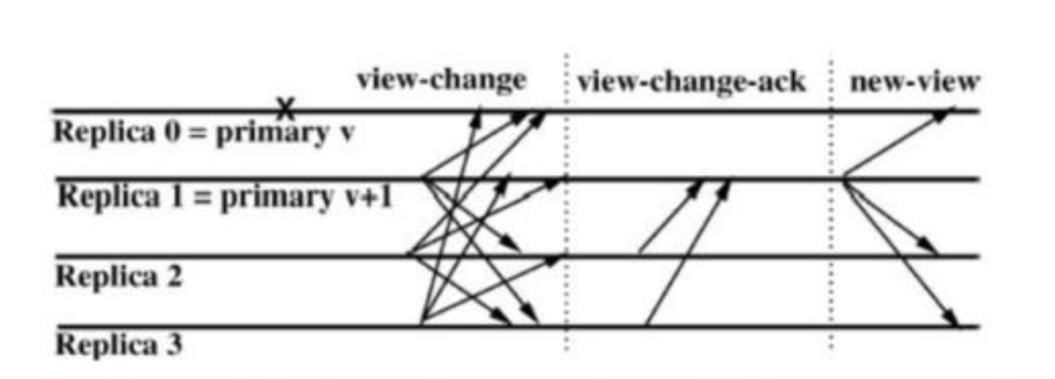
\includegraphics[width=0.8\textwidth]{figures/ch9/ch9_pbft_view_change.png}
\caption{PBFT View-change 视图切换协议}
\end{figure}

\begin{figure}[htbp]
\centering
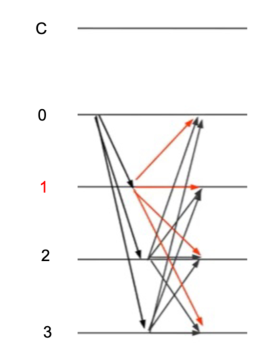
\includegraphics[width=0.8\textwidth]{figures/ch9/ch9_pbft_vs_paxos.png}
\caption{PBFT 与 Paxos 对比}
\end{figure}

% 图片：<!-- image -->，请替换实际路径
%\includegraphics[width=0.8\textwidth]{../work/figures/placeholder}

% 图片：<!-- image -->，请替换实际路径
%\includegraphics[width=0.8\textwidth]{../work/figures/placeholder}

\subsection{End of PBFT}


\chapter{Raft}
% <!-- image -->

\begin{center}
\begin{tabular}{ll}
\toprule
Request & Response \\
\midrule
// 33042 BPP & 7 s\#x42 = RPC Response \\
\bottomrule
\end{tabular}
\end{center}

% <!-- image -->

如果 Candidate 获得了多数派的选票，说明该 Candidate 在整个集群中拥有最新的日志（比多数派成员更加完整），或者和多数派成员的日志一样完整。该 Candidate 收到的选票来自集群中拥有最完整日志的任意一个成员。

\subsubsection{领导者选举}

请求投票 RPC 的请求与响应结构体：

\begin{verbatim}
type RequestVoteRequest struct {
    term         int  // 候选人的任期号
    candidateId  int  // 请求选票的候选人的 ID
    lastLogIndex int  // 候选人的最后日志条目的索引
    lastLogTerm  int  // 候选人的最后日志条目的任期
}
\end{verbatim}

\begin{verbatim}
type RequestVoteResponse struct {
    term        int   // 当前任期号
    voteGranted bool  // 如果候选人获得选票则为真
}
\end{verbatim}

Cand 收到某个成员的消息：
\begin{itemize}
\item 若该成员的任期号大于自己的任期号，说明该成员已经晋升为 Leader，则 Candidate 变为 Follower；
\item 若该成员的任期号小于自己的任期号，可能是迟到的前任 Leader 的心跳，则忽略并继续 Leader 选举流程。
\end{itemize}

领导者选举：一个稳定的 Leader 一旦选出，就不希望进行非必要的 Leader 变更。Raft 给出了以下不等式，只要系统满足，就能选举并维护一个稳定的 Leader：

\[
\text{broadcastTime} \ll \text{electionTimeout} \ll \text{MTBF} \quad (\text{MTBF, Mean Time Between Failure})
\]

\subsection{主要内容}

\begin{enumerate}
\item 基本概念
   \begin{itemize}
   \item Term 任期
   \item 三状态机及其转换
   \item 复制状态机
   \item RPC 通信
   \end{itemize}
\item 领导者选举
\item 日志复制
\item 性能分析与优化
\item Raft 优化
\end{enumerate}

\subsubsection{日志复制}

Leader 被选出来后，怎么知道新 leader 是哪个？若正好为 leader，就可以直接开始为客户端请求提供服务，执行指令即可。

若为 follower，通过心跳告知 leader。当节点宕机，client 尝试另一个节点；接收到客户端请求的节点若知道 leader 的 ID，会将请求转发给 leader。Leader 将指令作为新的日志条目，附加到本地日志，然后复制到 followers。当该条目被超过半数 follower 复制后，leader 可以提交该条目，并应用到自己的状态机，最后把结果返回客户端。

日志结构：每条日志包含指令、任期号和日志索引号（单调递增）。一个日志索引号和任期号唯一确定一条日志。

% 图示: 日志复制过程示意
\begin{center}
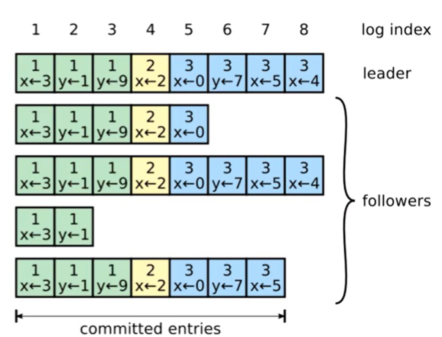
\includegraphics[width=0.8\textwidth]{figures/ch10/ch10_log_replication.png}
\end{center}

怎么让 follower 追上 leader，且所有节点的日志都完整且顺序一致？三种引起不一致的情况：
\begin{itemize}
\item follower 缓慢
\item follower 宕机
\item leader 宕机
\end{itemize}

Raft 通过一致性检查来处理：
\begin{itemize}
\item 若 follower 的日志中找不到 \texttt{prevLogIndex} 对应的条目，则拒绝此次 \texttt{AppendEntries RPC}；
\item Leader 收到拒绝后，逐步减小 \texttt{nextIndex}，重新发送，直到找到第一个二者一致的日志位置，然后复制该位置之后的所有条目；
\item Follower 中与 leader 冲突的日志条目会被 leader 的日志覆盖。因尚未提交，不违背一致性。
\end{itemize}

\textbf{一致性检查与冲突处理示例}

% 图示: 一致性检查与冲突处理
\begin{center}
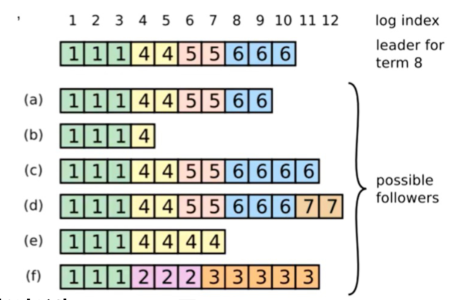
\includegraphics[width=0.8\textwidth]{figures/ch10/ch10_consistency_check.png}
\end{center}

右图最上面是当前 leader，此时 follower 中的 c 和 d 虽然比 leader 多出两个日志条目，但因为这些日志没有提交，所以不会产生冲突；leader 依靠自己的日志和选票当选（f 也可能投票给它）。多出的日志在冲突处理时会被覆盖。节点 f 拥有任期 2、3 的日志，大概说明它在那个任期内担任过 leader，但日志没有正常复制到大多数节点，也未提交。

若 leader 宕机，a、c、d 有机会成为新 leader。如果 c 或 d 当选，就可以将自己多出的日志复制给其他节点，从而使那些日志得到提交。老 leader 从宕机恢复后会成为 follower，其未提交的日志与新 leader 的日志发生冲突，通过一致性检查逐步回退，覆盖冲突内容。

追加日志 RPC 的请求与响应结构体：

\begin{verbatim}
type AppendEntriesRequest struct {
    term         int     // leader 的当前任期号
    leaderId     int     // leader 的 ID
    prevLogIndex int     // 新日志条目之前条目的索引
    prevLogTerm  int     // prevLogIndex 对应条目的任期
    entries      []byte  // 日志条目数据（为空时是心跳）
    leaderCommit int     // leader 已提交的最高日志索引
}
\end{verbatim}

\begin{verbatim}
type AppendEntriesResponse struct {
    term    int   // follower 的当前任期号
    success bool  // 若 follower 包含匹配 prevLogIndex 和 prevLogTerm 的条目则返回 true
}
\end{verbatim}

\begin{itemize}
\item \texttt{leaderCommit}：leader 确认日志被复制到大多数节点后才会提交 (Commit)，应用到自己的状态机，并通过 \texttt{leaderCommit} 字段将提交信息告知 followers。
\item Follower 收到提交信息后，会将自己已复制但未提交的日志标记为已提交，并应用到自己的状态机。
\item \texttt{response success}：只有 request 的 \texttt{term} 大于等于自己的 \texttt{term}，且通过一致性检查时，才返回 \texttt{true}；否则返回 \texttt{false}。
\end{itemize}

\textbf{日志复制：Summary}

\begin{itemize}
\item 一致性检查机制：leader 当选后无需特殊操作即可使日志恢复到一致状态，只需进行正常的 \texttt{AppendEntries} 操作；leader 从不会覆盖或删除自己的日志条目 (Append-Only)。
\item 只要过半数服务器能正常运行，Raft 就能接受并应用新日志条目，正常选出 leader 并提交日志。
\item 正常情况，新日志条目可在一次 RPC 来回中被复制到过半数机器；单个运行慢的 follower 不会影响整体性能。
\end{itemize}

\subsubsection{性能分析与优化}

基本任务：基于共识完成系统，通过 AppendEntries RPC 复制日志。理想情况下一次 RPC 即可。优化方法：
\begin{itemize}
\item \textbf{Batch（批量）}：一次网络开销可包含多个日志条目。
\item \textbf{Pipeline（流水线）}：leader 复制日志时不必等待 follower 回复，可连续发送后续 RPC。
\item 合理设置选举超时时间，平衡批量提交与延迟。
\item \textbf{Multi-Raft}：当数据量很大时，单个 Raft 的同步会成为瓶颈。可将数据划分为多个组，每组独立组成 Raft 集群，分别进行复制。但实现具有复杂性，例如如何做到负载均衡。
\end{itemize}

\subsubsection{Raft 优化}

% 原有空列表1-4，此处忽略，直接列出优点
\begin{itemize}
\item Raft 使用随机计时器进行 leader 选举，能够简单快速地实现。
\item Raft 保证首先选举出的 leader 必须拥有完整日志。
\item Raft 采用顺序日志复制的方法来避免日志空洞（非连续空洞）。
\item Raft 保证时刻都有具备完整日志的节点，可以成为 leader。
\end{itemize}

[疑似: \textbf{简单性/Simplicity}] 是 Raft 得以广泛认可与应用的关键。

% <!-- image -->

\subsection{End of Raft}


\chapter{Algorand与PoW}
Pure Proof of Stake in detail: The Algorand consensus is reached in three mandatory phases, plus one optional phase:

\subsection{Algorand 共识由三个强制性阶段和一个可选阶段达成:}

\begin{enumerate}
    \item Block proposal 区块提议
    \item Soft Vote 软投票
    \item Certify Vote 验证投票
    \item Recovery mode [疑似: 恢复模式]
\end{enumerate}

\subsection{The first phase: Block Proposal 第一阶段: 区块提案}

第一阶段，选出多个向网络提议新区块的账户，两个步骤:

\begin{itemize}
    \item \textbf{第一步: 选账户}
    \begin{itemize}
        \item 由 SPP 管辖、具有有效参与键的每个在线账户，运行 VRF，决定此账户是否被选中来提议区块。
        \item 拥有 Algos (代表权益) 数量越多，被选中概率越大。
        \item 可对每个 Algo 运行一次 VRF —— VRF 作用如同加权抽彩。
        \item 一旦某账户被 VRF 选中，节点将在网络中传播提议区块和 VRF 的输出。
    \end{itemize}
    \item \textbf{第二步: 广播验证}
    \begin{itemize}
        \item 后者用于证实提议者的有效性。
    \end{itemize}
\end{itemize}
进入软投票阶段。

\subsection{The second phase: Soft vote 第二阶段: 软投票}

此阶段目的是过滤提案，只保证一个区块获得认证。
\begin{enumerate}
    \item \textbf{Soft vote committee 选出软投票委员}

    每个节点对其管理的每个参与共识帐户重新运行 VRF，以抽选软投票委员会。基于账户拥有的 Algo 数量进行加权抽彩。

    \item \textbf{Voting 委员投票}

    每个节点都会从其他节点获得许多提议消息。如果它是委员会成员，它将在网上进行加权投票。节点验证，并用 VRF 和凭证验证有效性。节点将选择通过验证的最小散列凭证，并传播其提议区块 (最小散列凭证 + 提议区块)。此过程将持续一个固定时间，以便投票在网络中传播。此过程需要运行多次，直到多数派 (法定人数) 支持。最后进入认证投票阶段。
\end{enumerate}

\subsection{The third phase: Certify vote 第三阶段: 认证投票}

\begin{itemize}
    \item 抽选认证委员会:
    再次通过 VRF 抽选一个新委员会。同样每个节点遍历其管理的账户以选出委员会。
    \item 新委员会必须检验软投票阶段提出的区块: 检验是否存在双花，或任何其他问题。
    \item 如果有效，新委员会进行投票 (加权投票) 来认证该区块。
    \item 每个节点收集验证投票 (通过 VRF)，直到达到法定人数，触发此轮结束，为区块创建证书，并将其广播到网络。
    \item 开始新一轮共识流程，如此无限反复。
\end{itemize}

\subsection{Algorand 共识过程}

交易发送到交易区块上链的步骤:
\begin{enumerate}
    \item 从 Algorand 创建交易，并将其发送到网络;
    \item 一个节点接收交易后，通过八卦协议在网络上进行传播;
    \item 每个节点都会将一组交易放在一个新块中;
    \item 一轮共识开始;
    \item 区块提议;
    \item 软投票;
    \item 认证投票;
    \item 共识结束;
    \item 结束;
    \item 开始新一轮共识。
\end{enumerate}

\subsection{Algorand: 主要亮点}

\begin{itemize}
    \item Proof of Stake based Cryptocurrency
    \item 基于权益证明的加密货币
    \item High throughput: $\sim$1 min to confirm transactions vs an hour in Bitcoin
    \item - [疑似: Low latency: ...]
    \item Public ledger with low probability of forks
    \item 公共分类账: 分叉概率低
    \item Assumes 2/3-honest stake majority
    \item 假设 2/3 诚实的多数股权 (权益)
    \item Uses a gossip communication protocol
    \item 使用八卦通信协议
\end{itemize}


\chapter{分布式文件系统}
\section{分布式文件系统：目标与挑战}

文件系统基本功能：
\begin{itemize}
    \item 组织、存储、提取、管理内容+属性
    \item 命名、共享、保护文件 （类型、创建时间、权限等）
\end{itemize}

分布式场景核心需求：
\begin{itemize}
    \item 透明性 (Transparency)：访问远程文件如同本地
    \begin{itemize}
        \item 位置透明性 (Location Transparency)
        \item 位置无关性 (Location Independence)：名字解析由目录结构实现（路径名）
    \end{itemize}
\end{itemize}

核心挑战：
\begin{itemize}
    \item 网络延迟与故障
    \item 并发访问一致性
    \item 缓存协调
    \item 容错与状态管理
\end{itemize}

\section{1 抽象模型与设计问题}

\subsection{分布式文件系统抽象模型}

\subsubsection{1. 客户端}
\begin{itemize}
    \item 发起文件操作请求
    \item 可能进行本地缓存
\end{itemize}

\subsubsection{2. 服务器端}
\begin{itemize}
    \item 目录服务：路径名 + UFID 映射
    \item 文件服务：操作文件内容与属性
    \item 客户请求 → UFID (Unique File Identifier) → 服务器
\end{itemize}

\subsubsection{3. 通信}
\begin{itemize}
    \item 网络与基于 RPC
    \item 客户端与服务器
\end{itemize}

\textbf{思考}：UFID 应包含哪些信息？为何不直接用路径名作标识？(提示：防 rename race、支持 snapshot \& migration)

\subsection{分布式文件系统设计问题 (1/5)}

\subsubsection{1. 文件使用模式（经验、数据驱动设计）}
\begin{itemize}
    \item 多数文件长度 < 10KB
    \item 寿命短（临时文件）
    \item 多数文件性全本地暂存 + 普通数据
    \item 能被文件可共享 → 需一致性保障
\end{itemize}

\subsubsection{2. 命名与名字解析}
\begin{itemize}
    \item 构造名字空间（矩形、图、全局？局部？）
    \item 解析机制：路径遍历 vs. 缓存 vs. 委托
\end{itemize}

\subsection{分布式文件系统设计问题 (2/5)}

\subsubsection{3. 结构与接口}
\begin{itemize}
    \item 远程访问模型 (Remote Access)：操作粒度为 block/byte (NFS)
    \item 上载/下载 (Upload/Download)：下载/上传整个文件 (早期)
\end{itemize}

\subsection{分布式文件系统设计问题 (3/5)}

\subsubsection{4. 缓存策略与一致性}

客户端缓存一致性是指一套管理协议或规则，目的是在客户端本地访问速度与全局数据一致性之间寻求平衡。如果客户端总是直接读/写服务器，性能会很差；如果客户端只读/写本地缓存，又会出现数据不一致。

客户端缓存一致性策略：
\begin{itemize}
    \item Write-Through（直写）
    \item Delayed Write（延迟写）
    \item Write-on-Close（关闭写） (NFS 默认)
    \item Centralized Control（集中控制）
\end{itemize}

\subsubsection{Write-Through（直写）}
机制描述：客户端修改缓存数据的同时，直接同步到服务器端。
核心特点：
\begin{itemize}
    \item 数据一致性极高：服务器始终保持最新状态。
    \item 缺点：延迟较高，每次写操作都严重受限于网络带宽与延迟，性能开销大。
    \item 适用场景：对数据安全性要求极高的场景。
\end{itemize}

\subsubsection{Delayed Write（延迟写）}
机制描述：仅更新本地缓存，服务器端的同步操作被推迟到稍后时刻进行（如定时或缓冲区满）。
核心特点：
\begin{itemize}
    \item 性能极高：大部分写操作在本地内存完成。
    \item 一致性风险：若客户端在刷新到磁盘前崩溃，数据将丢失。
    \item 缺点：存在不可靠性，不适用于关键业务数据。
    \item 适用场景：对性能要求极高，且允许少量数据丢失的临时环境。
\end{itemize}

\subsubsection{Write-on-Close（关闭写）}
机制描述（NFS 默认策略）：文件打开期间的所有修改仅在本地，只有在执行 close() 操作时才将所有修改刷回服务器。
核心优势：
\begin{itemize}
    \item 平衡了性能与一致性：减少了频繁的网络交互。
    \item 符合应用习惯：符合“打开-编辑-保存”的常规流程。
\end{itemize}
潜在局限：
\begin{itemize}
    \item 若多客户端并发修改，在关闭前可能产生数据冲突或读到过期数据。
\end{itemize}

\subsubsection{Centralized Control（集中控制）}
机制描述：由服务器进行统一管理（如租约 Lease 或回调 Callback 机制），客户端遵循服务器指令。
核心特点：
\begin{itemize}
    \item 提供强一致性：支持原子操作。
    \item 动态管理：服务器可随时通知客户端作废旧缓存。
\end{itemize}
挑战：
\begin{itemize}
    \item 实现复杂，服务器开销大（需维护客户端状态）。
    \item 适用场景：共享在线系统、分布式数据库。
\end{itemize}

\subsection{分布式文件系统设计问题 (4/5)}

\subsubsection{5. 文件共享语义}
定义了多个客户端同时访问和修改时，如何处理读/写操作以保证“预期”的数据行为。
\begin{itemize}
    \item UNIX 语义：顺序一致性 (Sequential Consistency)
    \item 会话语义 (Session Semantics)：修改仅本地会话内可见。
    \item 事务语义：原子性保证。
\end{itemize}

\subsubsection{UNIX 语义 (Sequential Consistency)}
核心定义：基于本地文件系统的标准模型，提供顺序一致性。
机制：写操作立即生效，对所有用户可见。
行为：任何进程执行 write() 后，随后任何进程执行 read() 均能立即读到最新修改。
优点：编程模型简单，符合直觉。
缺点：分布式环境下性能极低（频繁网络通信）。

\subsubsection{会话语义 (Session Semantics)}
核心定义：一种折中方案，修改仅在当前会话内。
机制：
\begin{itemize}
    \item 修改仅在本地缓存进行。
    \item 关闭文件 (close) 时修改才同步回服务器。
    \item 打开文件 (open) 时才能获取最新更新。
\end{itemize}
典型应用：NFS (Network File System)。
优点：大幅减少网络交互，性能优异。
问题：存在“最后写者胜出”冲突。

\subsubsection{事务语义 (Transaction Semantics)}
核心定义：基于 ACID 原则的强一致性模型。
机制：所有操作视为一个原子事务。
特性：
\begin{itemize}
    \item 原子性：要么全成功，要么全失败。
    \item 中间状态不可见：直到 commit 提交为止。
\end{itemize}
技术支撑：通常依赖锁机制 (Locking) 或版本控制。
场景：分布式数据库、协同编辑系统。

\subsubsection{总结与对比}
\begin{center}
\begin{tabular}{lcc}
\toprule
语义 & 可见性/一致性 & 性能 \\
\midrule
UNIX & 立即 & 低 \\
会话 & 关闭时 & 高 \\
事务 & 提交时 & 低/中 \\
\bottomrule
\end{tabular}
\end{center}
选择原则：
\begin{itemize}
    \item 追求简单与一致 → UNIX 语义
    \item 追求高吞吐性能与 → 会话语义
    \item 追求强一致性和有严格要求 → 事务语义
\end{itemize}

\subsection{分布式文件系统设计问题 (5/5)}

\subsubsection{6. 断开操作与容错}
\begin{itemize}
    \item 有状态 vs. 无状态服务
    \item 服务器多副本 (Replication)
    \item 断开操作 (Disconnected Operation)
\end{itemize}

\subsubsection{服务模式：有状态 vs 无状态}

\textbf{无状态服务 (Stateless)}：服务器不保存客户端的信息（如打开的文件、锁）。\\
优势：容错简单，服务器崩溃重启后无需恢复状态。\\
挑战：每次请求都需包含完整上下文，可能增加开销。

\textbf{有状态服务 (Stateful)}：服务器记录客户端行为（如租约、打开的文件描述符）。\\
优势：性能更优，减少通信量。\\
挑战：故障恢复复杂，需精密的“状态重建”机制。

\subsubsection{服务器多副本 (Replication)}
核心目标：高可用性 (High Availability)：通过在不同节点存储多份数据，防止单点故障导致的数据丢失或服务不可用。

同步策略：
\begin{itemize}
    \item 强一致性：写操作需同步至所有副本（如 Paxos, Raft 协议）。
    \item 最终一致性：允许副本间短时延迟，通过后台异步同步。
\end{itemize}

技术挑战：
\begin{itemize}
    \item 副本间的数据不一致（Split-Brain 脑裂）。
    \item 写入性能下降（需等待多数派写入成功）。
\end{itemize}

\subsubsection{断开操作 (Disconnected Operation)}
定义：指客户端在网络不可用（或主动断开）的情况下，仍能使用读取/写访问。

关键技术：
\begin{itemize}
    \item Hoarding (预存)：在联网时先将可能使用的文件缓存到本地。
    \item Local Logging：断网期间所有修改记录在本地日志中。
    \item 重连挑战 (Reintegration)：
    \begin{itemize}
        \item 如何处理断网期间的修改冲突？
        \item 需通过版本控制或语义化合并来解决数据冲突。
    \end{itemize}
\end{itemize}

\subsubsection{权衡总结}
\begin{center}
\begin{tabular}{ll}
\toprule
设计重点维度 & 权衡 \\
\midrule
状态化 & 性能 vs 容错难度 \\
副本 & 可用性 vs 一致性成本 \\
断开 & 灵活性 vs 冲突处理复杂 \\
\bottomrule
\end{tabular}
\end{center}

原则：
\begin{itemize}
    \item 容错性往往以牺牲一部分写入性能为代价。
    \item 复杂的断开操作支持（如 Coda 文件系统）通常为已提升可用性。
\end{itemize}

\section{三、网络文件系统 NFS}

\begin{itemize}
    \item Sun 开发，事实标准
    \item POSIX 兼容
    \item 基于远程文件访问模型
    \item 通信：RPC
    \item 接口标准化：VFS (Virtual File System)
    \begin{itemize}
        \item 隐藏底层差异
        \item 本地操作 → 本地 FS
        \item 远程操作 → NFS
        \item VFS 接口上的操作或 client stub 下 server stub 传送到本地文件系统，或传送到 NFS 客户端的桩上（负责处理对存储在远程服务器上文件的访问，该访问通过 RPC 实现的）。
        \item 用户桩发出 RPC 调用
    \end{itemize}
\end{itemize}

\subsection{系统关键对象}
\textbf{文件句柄 (File Handle)}：服务器分配的不透明标识符。\\
客户端：解析路径 → 获取句柄 → 后续操作均使用句柄。\\
支持硬链接、符号链接。

\subsection{VFS}
% VFS 内容占位

\subsection{NFSv3 vs NFSv4}
\begin{center}
\begin{tabular}{lcc}
\toprule
操作 & NFSv3 & NFSv4 \\
\midrule
Create & $\checkmark$ & $\checkmark$ \\
Link & $\checkmark$ & $\checkmark$ \\
Symlink & $\checkmark$ & $\checkmark$ \\
Mkdir & $\checkmark$ & $\checkmark$ \\
Mknod & $\checkmark$ & $\checkmark$ \\
Rename & $\checkmark$ & $\checkmark$ \\
Remove & $\checkmark$ & $\checkmark$ \\
Rmdir & $\checkmark$ & $\checkmark$ \\
Open & $\times$ & $\checkmark$ \\
Close & $\times$ & $\checkmark$ \\
Lookup & $\checkmark$ & $\checkmark$ \\
\bottomrule
\end{tabular}
\end{center}

\subsection{文件句柄演进}

\textbf{持久文件句柄 (Persistent FileHandle)}：
\begin{itemize}
    \item 生命期内固定
    \item 对象删除/FS 卸载后失效
\end{itemize}

\textbf{挥发性句柄 (Volatile Handle, NFSv4)}：
\begin{itemize}
    \item 可随时失效（服务器可控）
    \item boot-time 结构：[vol=1|slot] slot：句柄表索引；
\end{itemize}

\subsection{NFS 命名与安装}

\subsubsection{1. 名字空间}
\begin{itemize}
    \item 服务器“导出”(export)
    \item 客户端“挂载”(mount) 到本地挂接点 (mount point)
    \item 可只挂载子树（非整个文件系统）
\end{itemize}

\subsubsection{安装协议}
远程文件安装协议：选定的挂接点。\\
服务器提供一组过程，由客户调用在本接点实现远程文件安装。

\subsection{NFS 文件属性}
可以用数据结构、布尔值、无符号整数或其他表示：
\begin{itemize}
    \item 强制属性 (Mandatory Attribute) --- 文件系统实现时必须支持
    \item 推荐属性 (Recommended Attribute)
    \item 命名属性 (Named Attribute)
\end{itemize}

\subsection{NFS 复合调用 (Compound Calls, NFSv4)}
将一系列操作合并为一个 RPC 调用以减少延迟。\\
(如：LOOKUP, OPEN, READ, WRITE, GETATTR 等)

属性列表：
\begin{itemize}
    \item object type：对象类型
    \item filehandle expiration：文件句柄过期时间
    \item change indicator：修改指示
    \item size：大小
    \item unix link support：UNIX 硬链接支持
    \item unix symlink support：UNIX 符号链接支持
    \item named attr：命名属性
    \item fsid：文件系统标识符
    \item lease duration：租用期限（秒）
    \item unique handle：唯一句柄
    \item readdir error：readdir 时返回的错误
    \item filehandle：文件句柄
    \item [generation]：防过期引用
\end{itemize}

操作说明：
\begin{itemize}
    \item CREATE：创建一个常规文件
    \item CREATE (特殊)：创建一个非常规文件
    \item LINK：创建一个文件的硬连接
    \item SYMLINK：创建一个文件的符号连接
    \item MKDIR：在给定目录下创建一个子目录
    \item MKNOD：创建一个特殊文件
    \item RENAME：更改文件名
    \item REMOVE：从文件系统删除一个文件
    \item RMDIR：从一个目录中删除一个空的子目录
    \item OPEN：打开一个文件
    \item CLOSE：关闭一个文件
    \item LOOKUP：根据文件名搜索文件
\end{itemize}

\subsection{持久文件句柄的格式}
\texttt{[文件系统标识符 | 文件 inode | inode 生成号 | ...]}

\subsection{VFS 层架构}
\begin{verbatim}
应用层
  |
VFS 层
  |
客户桩 --------- 服务桩
  |              |
本地文件接口    远程 SCSI 或 FC_SAN
\end{verbatim}

\subsection{NFS 远程过程调用与安全语义}

\subsubsection{1. RPC 重传}
客户发出一个 RPC 请求，并启动计时器。如果计时器超时，客户还没有收到响应，客户便使用原先相同的 XID (事务标识符) 重传原先的请求。如果文件服务器还没有处理完请求，服务器只需简单地忽略这个重传的请求。服务器通过 XID + 响应缓存实现 at-most-once 语义。

\subsubsection{2. 安全机制}
\begin{itemize}
    \item v2/v3：UNIX auth、Kerberos、Diffie-Hellman 密钥交换
    \item v4：RPCSEC\_GSS (通用安全服务 API)
    \begin{itemize}
        \item 支持多种安全机制 (Kerberos v5, SPKM, LIPKEY)
    \end{itemize}
\end{itemize}

\subsection{NFS 文件共享与加锁}

\subsubsection{1. 文件加锁}
\begin{itemize}
    \item NFS v2/v3：依赖独立协议 NLM (Network Lock Manager)
    \item NFS v4：内建加锁操作 (LOCK, LOCKU, LOCKT, RENEW)
\end{itemize}

\subsubsection{2. 访问控制}
每项指定用户/组 + 权限位 (read/write/execute/…)

% image: 图片路径未提供，保留注释

\subsection{NFS 缓存、委托与复制 (1/2)}

\subsubsection{1. 客户端缓存一致性}
\begin{itemize}
    \item 数据可缓存 (read/write)
    \item Write-on-Close：关闭时回写
    \item 缓存重验证 (Revalidation)：
    \begin{itemize}
        \item 重开已缓存文件时；比对 mtime / ctime
        \item 过期则丢弃缓存
    \end{itemize}
\end{itemize}

% image: 图片路径未提供，保留注释

\subsection{NFS 缓存、委托与复制 (2/2)}

\subsubsection{2. 委托 (Delegation, NFSv4)}
\begin{itemize}
    \item 服务器将责任委托给客户端
    \item READ delegation：客户保证期间无人写
    \item WRITE delegation：客户保证期间无人读/写
    \item 权衡：性能提升，但服务器故障时状态恢复复杂度增加（有状态代价）
\end{itemize}

\subsubsection{3. 服务器复制与迁移}
复制：仅支持整个文件系统级复制（逻辑设备）。由于复制情况下，客户在服务器之间的切换不受服务器控制，状态信息的处理是不同的。

迁移：用于负载均衡，需迁移全部状态，所有服务器状态要从原服务器传送到新服务器。NFSv4 对文件复制只提供最低限度的支持。只有整个文件系统可以被复制（包括文件、属性、目录和数据块组成的逻辑设备）。

\medskip
汇报完毕，欢迎同学们批评指教！本次课内容教材上没有。


\chapter{分布式事务}
\input{sections/ch13_converted.tex}

\end{document}
